% =====================================================================
%  Journal of Cheminformatics — Research article
%  Formatted to BMC/Springer Nature submission guidelines:
%    double-line spacing, line and page numbering, no page breaks,
%    single column, Springer author-year reference style.
%  Compile: pdflatex -> bibtex -> pdflatex -> pdflatex
%
%  REVISION 2026-09-27
%    - Added Sections 2.8 and 3.6: independent ChEMBL re-retrieval and
%      chemotype stratification of the assay-modality offset.
%    - Softened the DAT-versus-SERT claim (see Limitations).
%    - Added Fooladi et al. 2025 to the scaffold-splitting literature.
%    - Removed a duplicated \maketitle after the abstract.
% =====================================================================
\documentclass[11pt,a4paper]{article}

\usepackage[margin=2.5cm]{geometry}
\usepackage[expansion=false]{microtype}
\usepackage{setspace}
\usepackage[mathlines]{lineno}
\usepackage{booktabs}
\usepackage{graphicx}
\usepackage{amsmath}
\usepackage{siunitx}
\usepackage{caption}
\usepackage{placeins}
\usepackage[round]{natbib}
\usepackage[hidelinks]{hyperref}
\usepackage{pgfplots}
\pgfplotsset{compat=1.18}
\usepgfplotslibrary{groupplots}

\doublespacing
\linenumbers
\bibliographystyle{plainnat}

\captionsetup{font=small,labelfont=bf,justification=justified,singlelinecheck=false}
\setlength{\parindent}{0pt}
\setlength{\parskip}{6pt}

\definecolor{cbBlue}{HTML}{0072B2}
\definecolor{cbVerm}{HTML}{D55E00}
\definecolor{cbGreen}{HTML}{009E73}
\definecolor{cbSky}{HTML}{56B4E9}
\definecolor{cbOrange}{HTML}{E69F00}
\definecolor{cbGrey}{HTML}{666666}
\definecolor{cbLGrey}{HTML}{BBBBBB}

\pgfplotsset{
  papershared/.style={
    width=0.8\linewidth, height=5cm,
    tick align=outside, tick pos=left,
    axis line style={very thin,black!70},
    grid=major, grid style={black!10,very thin},
    label style={font=\small}, tick label style={font=\scriptsize},
    legend style={font=\scriptsize,draw=none,fill=none},
    title style={font=\small\bfseries,align=left},
  }
}

\title{\bfseries A NET binding-versus-functional potency offset is a property of the
assay cell, not of the assay format: consequences for external validation of monoamine
transporter models}

\author{Selim Emin Sahin\,$^{1,2,*}$}
\date{}

\begin{document}
\maketitle

\noindent$^{1}$Department of Chemistry, The University of Texas at Austin, Austin,
Texas 78712, United States\\
$^{2}$Department of Neuroscience, The University of Texas at Austin, Austin,
Texas 78712, United States\\[4pt]
$^{*}$Corresponding author: Selim Emin Sahin, \href{mailto:selimeminsahin@utexas.edu}{selimeminsahin@utexas.edu}

\section*{Abstract}

\textbf{Background.} Monoamine transporter activity models are almost universally
evaluated by cross-validation. Two quantities needed to interpret one --- the offset
between assay modalities, and the response region an external set samples --- are rarely
reported, and each is a property of the data rather than of the model.

\textbf{Methods.} We curated 24\,445 ChEMBL\_37 bioactivities into a censoring-aware
benchmark of 2849 compounds across 899 scaffolds and evaluated gradient-boosted models
over twenty scaffold-disjoint fold realisations. Assay modality and binding radioligand
were read from the free-text assay description, not from ChEMBL's
\texttt{assay\_type} field. The binding-versus-functional offset was decomposed by a
fixed-effects model with compound-within-document effects, then stratified by radioligand.
Models were tested under a protocol fixed in advance --- not externally registered ---
against 42 stimulants from one independent study.

\textbf{Results.} The binding-versus-functional offset at NET is not a property of the
assay format. Within compound and within document it is $+0.507$ in the 17 documents
using [$^{125}$I]RTI-55 as the NET radioligand and $+0.038$ in the 21 using
[$^{3}$H]nisoxetine; the pooled $+0.261$ is an average of the two. The same stratification
at DAT and SERT spans $-1.04$ to $+0.18$, so the offset is a property of the assay cell;
radioligand is collinear with chemotype here, so which feature is operative cannot be
settled. The external test failed its declared criterion and was powered only for DAT. Two validation diagnostics returned numbers their construction cannot support: an
outcome-conditioned error regression yields $R^{2}=0.444$ where a shrinkage null
reproduces 0.448 and its only pre-outcome form gives 0.001; and a composition-matched
comparator is unattainable in all nine target $\times$ set cells, though a rejection
sampler returns a band for every one.

\textbf{Conclusions.} Three numbers here that read as properties of a model or a
measurement format are properties of the set they were computed on. Report that composition --- which assay
cells, which response region --- alongside the score, and check a matched comparator is
attainable before interpreting it.

\textbf{Scientific Contribution.} We show that the binding-versus-functional potency
offset at NET is present in assays using one radioligand and absent from assays using
another, so it is not the assay-format effect it appears to be in pooled data, and that
the same stratification reveals a 1.2 log-unit spread across binding assays at the other
two transporters. The analysis rests on a reusable labelling of assay modality for
14\,386 human monoamine transporter records derived from assay free text, now carrying
measured precision against a blind annotation made under a stated rule. We further
demonstrate that two validation diagnostics for external error return
interpretable-looking numbers that their construction does not support, and supply the
shrinkage null and the attainability check against which each should be tested.

\begin{figure}[tb]
\centering
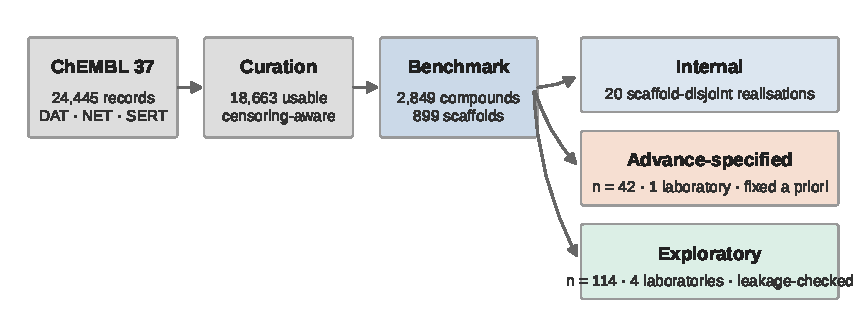
\includegraphics[width=\linewidth]{figures/fig1_design.pdf}
\caption{Study design. Flow from ChEMBL\_37 retrieval through censoring-aware
curation to the benchmark, and onward to its three evaluation arms. Only the second of
them --- the 42-compound external test --- was specified before any external potency value
was examined; the 114-compound extension was assembled afterwards and its endpoints were
not pre-specified. Two further external sets (PDSP/BindingDB, $n=17$,
and Cui et al., $n=20$) were assembled afterwards and are reported as an exploratory
extension in \S\,\ref{sec:newexternal}; they are not part of the advance-specified design.}
\label{fig:design}
\end{figure}

\section{Introduction}

The dopamine, norepinephrine and serotonin transporters (DAT, NET, SERT;
\textit{SLC6A3/2/4}) clear monoamines from the synaptic cleft and are the molecular
targets of psychostimulants, antidepressants and a continuously expanding set of novel
psychoactive substances. Their relative potencies determine pharmacological character:
compounds with a DAT/SERT inhibition ratio above 10 produce psychostimulant effects and
high abuse potential, while those below 0.1 produce entactogenic, MDMA-like effects. Both
numeric cut-points are stated together in the caption to Figure 1 of Luethi and Liechti's
2020 review.\cite{Luethi2020} The ratio itself is defined as 1/DAT\,IC$_{50}$ :
1/SERT\,IC$_{50}$ after \citet{Baumann2012}, and the qualitative direction --- DAT-selective
compounds stimulant-like, SERT-selective compounds entactogen-like --- is the older
result.\cite{Luethi2018}

Quantitative structure--activity models for these targets are typically evaluated by
cross-validation. Scaffold-based splitting, which confines all compounds sharing a
Bemis--Murcko scaffold \cite{Bemis1996} to a single partition, is widely regarded as the
conservative choice because it prevents analogue series from spanning the train/test
boundary.\cite{Sheridan2013,Lenselink2017} Recent work indicates that this expectation is
optimistic. Molecules assigned different Bemis--Murcko scaffolds are frequently
highly similar, so the split does not create the distribution shift it is assumed
to;\cite{Guo2024,Guo2025} across eight datasets, fourteen model families and ten
splitting strategies, scaffold-split performance was found not to differ
substantially from random splitting, whereas splitting on similarity clusters was
markedly harder and correlated far more weakly with in-distribution
performance.\cite{Fooladi2025} Two 2026 benchmarks reach the same conclusion from different directions: that the
interpolation-to-extrapolation penalty is a property of the data set rather than of
the algorithm,\cite{Alshehade2026} and that splitter choice changes what an
evaluation estimates far more than it changes which model wins.\cite{Crucitti2026}
This matters for the present work in a specific way:
Murcko abstraction discards ring substituents, which for this target family are the
determinants of selectivity, so scaffold identity is a coarse proxy for chemical
novelty here (see \S\,\ref{sec:scaffold-leak} and Limitations).

Scaffold splitting addresses one leakage pathway. It does not control for assay
heterogeneity, laboratory provenance, or the narrowing of response range that occurs
when a benchmark is assembled from historical literature.\cite{Landrum2023,Mayr2018} Whether scaffold-split
estimates predict performance on compounds measured elsewhere has not been established
for this target family, and the question is practically consequential: forensic and
regulatory users apply such models to newly emerging substances characterised in
laboratories other than those contributing the training data.

We test this directly. The model and evaluation endpoints were fixed before any
external value was examined, and the advance-specified result is reported unchanged
regardless of outcome. We then decompose the observed shortfall into contributions from
response range, chemotype, assay modality and test-source identity.

\section{Methods}
\label{sec:methods}

\subsection{Data source and curation}
\label{sec:data}
\begin{sloppypar}
Bioactivities were retrieved from the ChEMBL REST API (release ChEMBL\_37, released
2026-05-01; accessed 2026-09-08) for the human single-protein targets CHEMBL238 (DAT),
CHEMBL228 (SERT) and CHEMBL222 (NET), restricted to $K_i$ and IC$_{50}$ endpoints,
returning 24\,445 records.\cite{Zdrazil2024,Davies2015}
\end{sloppypar}

Records were removed if ChEMBL flagged a data-validity problem, if the assay type was
neither binding (B) nor functional (F), if a canonical SMILES was absent, or if units
were not nanomolar, leaving 18\,663 usable measurements. By ChEMBL's
\texttt{assay\_type} field 97.6\% of these derive from radioligand binding assays and
2.4\% from functional assays; \S\,\ref{sec:modality-labelling} shows that field to be
unreliable here and recovers a very different proportion from the assay text.
Structures were standardised with RDKit \cite{RDKit} and potencies converted to the
p-scale ($-\log_{10}$ molar).

The resulting endpoint is heterogeneous. It combines radioligand binding affinity
with functional uptake-inhibition potency, and pools transporter substrates with
pure reuptake blockers. The models therefore predict a ChEMBL-derived transporter
activity endpoint rather than a uniform mechanistic quantity, and
\S\,\ref{sec:assay-modality} quantifies
one consequence of that heterogeneity.

\subsection{Labelling assay modality from the assay description}
\label{sec:modality-labelling}
ChEMBL's \texttt{assay\_type} field does not separate radioligand binding from
functional uptake inhibition in this corpus: 8420 of the 8801 IC$_{50}$ records in the
re-retrieval described below are tagged \texttt{B}. Taken at face value the field implies that functional measurements
are 2.4\% of the data, on either corpus, and therefore too scarce to model, a conclusion that is an
artefact of the annotation rather than of the literature. It is more accurate to say that
the field under-recovers functional measurements than that it mislabels them: of the 403
records ChEMBL tags \texttt{F} in this corpus, 337 are functional uptake by the text, so
the tag is specific (84\%) but recovers 6\% of the 5601 functional records the text
identifies. These 403 are counted on the 16\,750-record re-retrieval and are not the same
quantity as the 2.4\% functional share of the 18\,663-record frozen set reported in
\S\,\ref{sec:data} (roughly 448 records); the two happen to land on similar fractions of
different corpora. \texttt{assay\_type} encodes how the source publication classified the assay,
which is a different question from what was measured, and the gap below should be read as
a definitional mismatch rather than as curation error.

\paragraph{Which corpus.} The labelling is computed on the independent re-retrieval of
\S\,\ref{sec:rederivation} (16\,750 records, 2026-09-27), not on the frozen ChEMBL\_37
benchmark of \S\,\ref{sec:data} (18\,663 usable measurements). The two counts are
different quantities and were previously reported without saying so. Every offset analysis
in \S\,\ref{sec:assay-modality}--\S\,\ref{sec:within-doc} is therefore computed on the
re-retrieval; the benchmark and all model fitting use the frozen set. The deposited
labelling table carries a provenance column.

Modality was therefore read from the free-text \texttt{assay\_description} by ordered,
high-precision regular expressions, independently of \texttt{standard\_type}. The
phrases \emph{uptake site} and \emph{reuptake site} are neutralised first, because
there the word names the target rather than the measurement; descriptions asserting
both modalities are placed in a \texttt{conflict} class and undecidable ones in an
\texttt{unclear} class, and both are excluded rather than guessed. Of 16\,750 records,
8785 classify as binding, 5601 as functional uptake, 810 as conflicting and 1554 as
undecidable --- so functional measurements are 39\% of the classifiable corpus, not
2.4\%. Per-target compound counts with functional data are 1216 (DAT), 1732 (NET) and
1774 (SERT).

This labelling is what makes the decomposition in \S\,\ref{sec:twobytwo} possible, and
it is deposited as a reusable table of 11\,693 (compound, target, modality) medians.
Automated and manually curated re-annotation of ChEMBL assay descriptions has recently
been pursued at corpus scale;\cite{Smit2026} the labelling here is narrower --- one
binary distinction over one target family. Its accuracy is measured rather than assumed.
A stratified random sample of 186 distinct assay descriptions was annotated from the text
alone, blind to the classifier's output, under the rule that a description counts as
binding only if the measurement is displacement of a named radioligand and as functional
only if it is inhibition of substrate transport, with everything else recorded as
undetermined. On the 130 sampled records the classifier actually emits --- it excludes the
\texttt{conflict} and \texttt{unclear} classes --- precision is 0.914 (95\% CI
0.825--0.960) for binding and 0.967 (0.886--0.991) for functional uptake, and overall agreement is 0.938
(0.883--0.968). Recall is 1.000 for both classes, but that figure is close to tautological
given the error structure and should not be read as perfect recall: it is computed only
over the records the annotation resolved. The informative property is the negative one. There is no case in the sample where the classifier assigns one modality
and the annotation reads the other; every disagreement is the classifier committing where the
annotation judged the text undetermined, and four of the eight arise from assay text that
describes a different target. The excluded classes behave as intended in one direction and
conservatively in the other: \texttt{unclear} is 36 of 40 genuinely undetermined, while
\texttt{conflict} is 11 of 16 recoverable functional records, so the exclusion discards
real functional data rather than admitting wrong labels. The annotation was produced by a
large language model under the stated rule and is deposited in full; it is a
reproducible-rule annotation, not an independent expert gold standard, and is reported as
such. Within-pair designs of this kind have been shown to be the robust way
to work across inter-assay variability.\cite{Nelen2025} The consequence of not
making the distinction has been stated for this target family: Lee et al.\ conclude
that it is ``not advisable to combine either $K_i$ and IC$_{50}$, or uptake and
binding data sets'' when modelling the dopamine transporter, while noting that the
direction of any such offset was undetermined.\cite{Lee2024}

\subsection{Separating assay format from value type}
\label{sec:twobytwo}
Because ChEMBL's binding records are predominantly $K_i$ and its functional records
predominantly IC$_{50}$, a comparison of ``binding $K_i$'' with ``functional
IC$_{50}$'' moves two things at once: the assay format and the value type, the latter
of which carries a Cheng--Prusoff relationship.\cite{Kalliokoski2013} With modality
labelled independently of \texttt{standard\_type} the two become separable, and the
off-diagonal cells are well populated (3018 binding IC$_{50}$ and 1336 functional
$K_i$ records).

Both effects were estimated in one model: pChEMBL regressed on an indicator for
functional modality and an indicator for $K_i$, with \textbf{compound-within-document
fixed effects} --- so every contrast is between assays run on the same compound in the
same publication --- and standard errors clustered on document, the unit that shares a
protocol, cell line and operator. Robustness was assessed by leave-one-document-out,
by moving the \texttt{conflict} class into each modality in turn, and by refitting with
document rather than compound-within-document effects.

\paragraph{Mechanism stratification.} To test whether the format effect is carried by
transporter substrates, for which $K_\mathrm{m}\neq K_\mathrm{D}$ is
expected,\cite{Schomig1988,Eshleman1999} compounds were classified as substrate-type
releasers or uptake blockers \emph{from structure alone}. Using the $K_i$/IC$_{50}$
ratio for this purpose would be circular, since that ratio is the quantity under test.
Blocker-defining motifs ($\alpha$-pyrrolidinophenone, tropane, aryloxy and diaryl
ether, piperazine, fused tricyclic, benzhydryl, $\alpha$- and $\beta$-ester,
$N$-\textit{tert}-alkyl) are applied first as hard negatives, then a molecular-weight
and ring-count gate, then substrate cores (arylethylamine, cathinone, constrained
amine, arylmorpholine, aminooxazoline, aminoindane). Against a 55-compound reference
set --- 28 substrate-type releasers and 27 uptake blockers, deposited in full with class
labels --- the rule achieves 96\% recall on releasers, 100\% specificity on blockers and
98\% balanced accuracy. The single miss is MDAI, a ring-constrained releaser caught by the
ring-count gate. A missed releaser contaminates the blocker stratum anti-conservatively,
so the blocker-only estimate of \S\,\ref{sec:within-doc} is a lower bound on how clean
that stratum is.

\subsection{Identifying the binding radioligand}
\label{sec:radioligand}
The same assay descriptions that carry the modality also name the radioligand. A second
set of ordered regular expressions extracts it, matching the specific ligands first ---
nisoxetine, desipramine, RTI-55 (with its synonym $\beta$-CIT), mazindol,
WIN\,35,428 (with CFT), citalopram, paroxetine, imipramine, cocaine and GBR\,12935 ---
before the native substrates norepinephrine, serotonin and dopamine, and recording
\texttt{unstated} otherwise. The radioligand is recovered
from 77--84\% of binding records at each target. A document is assigned to the stratum of
the radioligand it uses for the most records, and a stratum is reported only if it holds
at least five documents --- which excludes one cell, [$^{3}$H]mazindol at DAT (3
documents, 37 records, $-0.036$), whose inclusion would not change any statement made
here.

This was added during revision, in response to the observation that a NET-specific
discrepancy between binding and functional measurement has an obvious candidate cause that
is not the assay format: human NET binding is dominated by a small number of radioligands
whose nonspecific binding and whose $K_D$ in the Cheng--Prusoff conversion differ, and a
systematically mis-calibrated $K_D$ in one of them produces a constant shift in every
$K_i$ from that assay, at one target only. It is a text query on data already parsed, so
the hypothesis is testable without new experiments.

\subsection{Censoring}
Left-censored measurements were retained at their bounds. Exclusion is not neutral:
discarding censored records removes 672 compounds (23.6\%) non-randomly, with bounds
clustering at the 10\,\textmu M screening concentration and the discarded
population differing from the retained one at every target (Kolmogorov--Smirnov
$p\leq6\times10^{-95}$). Exclusion removes 189 scaffolds entirely and shifts the
selectivity class distribution ($\chi^2$, $p=1.6\times10^{-7}$), depleting the
psychostimulant-like class from 16.2\% to 7.9\%. Censored records are 18.2\%, 7.3\% and 10.5\%
of the DAT, NET and SERT columns, with a median bound of $p=5.00$ against uncensored
medians of 6.78, 6.89 and 7.13 --- they sit at the weak end, as the screening
concentration implies.

Retaining a bound as a point value is a benchmark-preserving convention, not an assertion
that the latent potency equals the bound. To bound what the convention costs, the same
pipeline was refitted with a censored objective that penalises predictions above the bound
and leaves predictions below it free ($L=\max(0,f-y)^2$ for censored records,
$L=(f-y)^2$ otherwise), over ten scaffold-disjoint realisations, scoring on uncensored
compounds only so that every label is a real value. Internal $r^2$ changes by $+0.007$
(DAT), $+0.003$ (NET) and $-0.001$ (SERT) and RMSE by $0.000$, $+0.001$ and $+0.002$; the
full table is deposited. The choice of loss is therefore not what any conclusion in this
paper rests on. Methods that treat censoring as more than a loss-function choice exist and
are not pursued here: Svensson et al.\ show that carrying censored labels through the
likelihood improves calibrated uncertainty rather than point accuracy, which is consistent
with the deltas above and is the direction in which this benchmark would benefit from
them.\cite{Svensson2025} (These $r^2$ values, 0.523/0.465/0.502 under squared loss, are not
comparable with Table~\ref{tab:internal}: they are computed on the uncensored subset
alone, which excludes the censored compounds clustered at the bound and is a harder set.)
\textbf{Final benchmark: 2849 compounds across 899 scaffolds.}

\subsection{Measurement reproducibility}
\label{sec:repro-floor}

\begin{table}[tb]
\centering
\small
\caption{Measurement reproducibility by target. Standard deviation and standard error
of the mean across replicate measurements of the same compound at the same target, in
log units.}
\label{tab:repro}
\begin{tabular}{lrrrr}
\toprule
Target & Groups & Median SD & Mean SD & Median SEM \\
\midrule
DAT  & 823   & 0.166 & 0.268 & 0.100 \\
NET  & 802   & 0.212 & 0.293 & 0.132 \\
SERT & 1032 & 0.194 & 0.296 & 0.137 \\
\midrule
All  & 2657 & \textbf{0.194} & 0.287 & \textbf{0.127} \\
\bottomrule
\end{tabular}
\end{table}

A replicate group is all records for one (compound, target) pair, taken across documents,
assay types and modalities, after the curation filters of \S\,\ref{sec:data}; the median
group holds 2 records and the 90th percentile holds 5. Table~\ref{tab:repro} reports the
median and mean of the per-group standard deviations, which describe the distribution of
agreement between replicates. Where an error \emph{variance} is needed rather than a
description --- in the ceilings of Table~\ref{tab:extceiling} --- we use the pooled,
degrees-of-freedom-weighted estimate instead, which is 0.444, 0.471 and 0.525 on these
same groups. It is larger than the median because a two-record group's standard deviation
is a low-biased estimate of the dispersion it is drawn from, and the pooled figure is the
one that estimates that dispersion. Because the groups span modalities,
the figures above are an upper bound on pure measurement error: they already contain part
of the assay-modality offset of \S\,\ref{sec:assay-modality}, which is why that offset is
compared against this floor rather than estimated from it. Restricting groups to a single
modality is not possible at useful sample size, since most compounds are measured one way
only.

These values sit close to the canonical estimate for heterogeneous public $K_i$ data:
Kramer et al.\ report a mean error of 0.44 and a standard deviation of 0.54 p$K_i$ units
across ChEMBL, after filtering for the unit-transcription errors, undifferentiated
stereoisomers and repeated citations that inflate naive estimates, and derive a maximum
attainable $R^2$ of 0.81 on large data sets.\cite{Kramer2012} Our 0.194 median SD is
smaller because it is computed within one target family and after the same class of
filtering, and our 0.820/0.633/0.838 internal ceilings are the same calculation applied
per target.

Because models predict the aggregated (median) value, the relevant comparator for model
error is the standard error of that aggregate, 0.127 log units.

\subsection{Descriptors, models and cross-validation}
Features were ECFP4 Morgan fingerprints \cite{Rogers2010} (radius 2, 2048 bits) with ten
physicochemical descriptors. Models were LightGBM \cite{Ke2017} gradient-boosted regressors (250 estimators, learning
rate 0.06, 31 leaves, minimum 10 samples per leaf, column subsample 0.4, fixed seed),
with hyperparameters fixed before external evaluation. They were not tuned: they are
LightGBM defaults except for the learning rate, leaf count and column subsample, which
were set once by inspection of scaffold-CV performance on an early version of the
benchmark and never revisited. No nested cross-validation was run. That early inspection
used the same kind of folds as the reported CV, so the internal estimate is a selected
rather than a clean one, and it is the comparator against which the external shortfall is
measured. We do not attempt to bound the optimism this
introduces, because fold-seed variation at fixed hyperparameters and variation over the
learning-rate, leaf-count and column-subsample grid are different spaces and the first
does not bound the second. The claim is the weaker and sufficient one: a selection over
three parameters, made once on an earlier version of the benchmark, cannot plausibly
account for shortfalls of 0.13--0.49. The optimism is not zero, and a shortfall of 0.02
would not survive it; these are not that. Five scaffold-disjoint folds
were generated with zero cross-fold scaffold overlap verified, repeated twenty times
with different scaffold orderings; internal figures are mean $\pm$ SD across those
realisations. Note that fingerprint features encode ring substitution, so substituent
information is available to the model even though it is discarded by the Murcko
abstraction used to define the folds.

\paragraph{Which $R^{2}$.} Two quantities share the symbol and they are not
interchangeable. Unless stated otherwise, values reported here as $R^{2}$ or $r^{2}$
are the \emph{squared Pearson correlation} between observed and predicted values, which
is the definition used throughout the analysis code. It is invariant to any linear
rescaling of the predictions and therefore measures agreement in ranking and spread
only. The coefficient of determination, $1-\mathrm{SS_{res}}/\mathrm{SS_{tot}}$,
additionally penalises predictions that are systematically shifted or compressed, and
is reported separately where the two diverge --- which on the external sets they do
substantially, because the predictions compress toward the training mean
(\S\,\ref{sec:decomp}). Both are tabulated for every external cell in the deposit.

\paragraph{Reproducibility of the primary analysis.}\label{sec:reimplementation} The internal pipeline was
re-implemented from the deposited source and re-run over twenty scaffold-disjoint
realisations. It reproduces Table~\ref{tab:internal} to within 0.003 in $r^{2}$ and
0.003 in RMSE at every target ($r^{2}$ 0.584 / 0.502 / 0.538 against 0.584 / 0.501 /
0.541; RMSE 0.736 / 0.811 / 0.887 against 0.735 / 0.811 / 0.884). The residual
difference is the fold-seed stream, not the model. Table~\ref{tab:internal} and every
external quantity in this paper are reported from the \emph{original} run; the re-run is
a check on it and is not mixed into any reported figure.

\subsection{External evaluation under an advance-specified protocol}
\label{sec:prereg-protocol}
The protocol below was written down before any external potency value was
examined, and the result is reported unchanged. It was \emph{not} registered
with any external registry, carries no third-party timestamp and no deposited
hash, so the claim is self-attested and a reader cannot verify it independently;
we use ``advance-specified'' rather than ``pre-registered'' throughout to mark
that distinction. Two amendments were made after the external values were seen; both
are declared inline below, in the places they apply.
\textit{Endpoints, ranked in advance:} (1) DAT/SERT log-ratio regression;
(2) selectivity classification; (3) per-target regression; (4) exploratory cross-target
error correlation. \textit{Exclusions:} as specified, compounds sharing a full InChIKey
with any training compound were removed. \textit{Deviation, declared:} during revision
this was tightened to the InChIKey \emph{skeleton block}, which is the correct unit for
this feature set because ECFP4 ignores stereochemistry --- a stereoisomer of a training
compound carries a different full key and an identical fingerprint. On the advance-specified
test the two rules are equivalent: both remove the same four compounds, 2Me-$\alpha$-PVP,
3Me-$\alpha$-PVP, cocaine and MDMA, so no advance-specified result turns on the change. It
is not equivalent on one of the exploratory sets added later, where it removes 13 further
compounds and lowers a reported $R^2$; that case is set out in
\S\,\ref{sec:newexternal}.
\textit{Success criteria:} external $R^2$ within 0.10 of internal $\rightarrow$
generalises; more than 0.20 below $\rightarrow$ generalisation failure, reported as a
finding. \textit{Test set:} 46 compounds from Stalberga et al.\cite{Stalberga2026}, of which 4
were excluded by either rule, leaving 42. \textit{Amendment, declared:} one of the 46
structures was found during revision to be the wrong molecule --- cocaine recorded as its
inactive hydrolysis metabolite benzoylecgonine --- and was corrected. Because the training
set holds ($-$)-cocaine, the corrected structure is caught by the overlap filter and the
wrong one was not, so the correction moved the test set from 43 compounds to 42. Both the
error and its two consequences are set out above. A cross-check of all 40 external
structures carrying PubChem identifiers found no further discrepancy beyond
free-base-versus-salt differences, which are intended. We note what this means for
the status of the protocol: a specification that can be amended after the outcome is known,
with no external timestamp to anchor the original, is weaker evidence than a registered one,
and we claim no more for it than that.

\paragraph{Exploratory extension.} After the advance-specified analysis was complete, the
external set was extended with the Luethi and Liechti compilation,\cite{Luethi2020} six
Basel primary studies,\cite{Simmler2013,Simmler2014,Rickli2015a,Rickli2015b,Luethi2019,Kolaczynska2019}
and Eshleman et al.\cite{Eshleman2017} Structures were resolved by two independent routes:
CAS registry lookup and OPSIN parsing of IUPAC names.\cite{Lowe2011} Analyses in
\S\,\ref{sec:extended} and \S\,\ref{sec:pilot} are exploratory.

\subsection{Use of large language models}
Analyses were designed, implemented and executed with assistance from a large
language model (Claude, Anthropic) acting as a coding and analysis collaborator. The
model did not author the manuscript and does not meet authorship criteria. All
numerical results reported here were produced by executed code and are reproducible
from the deposited repository. Implementation errors identified and corrected during
development are enumerated in the Declarations.

\subsection{Decomposition of external error}
Absolute prediction error was regressed on three predictor blocks: response-range
position (distance beyond the training interquartile range, zero inside it), chemical
similarity (nearest-neighbour Tanimoto to training), and source identity (dummy-coded
by study). Each block's \emph{unique} contribution is the drop in model $R^2$ when that
block alone is removed.

\subsection{Independent re-retrieval and chemotype stratification}
\label{sec:rederivation}
To test whether the assay-modality offset is an artefact of a single retrieval or of
a single chemotype, activities were retrieved again from the live ChEMBL REST API on
2026-09-27, sixteen months after the frozen ChEMBL\_37 release, using an
independently written curation script. Binding was taken as $K_i$ from assays ChEMBL
types \texttt{B}; functional as IC$_{50}$ from assays typed \texttt{F}; records were
restricted to human targets with a ChEMBL \texttt{pchembl\_value} present, an
uncensored relation, and no data-validity comment. Per compound and modality the
median was taken, and the offset defined as functional minus binding. This retrieval
returned 16\,750 records and yields a compound set that is \emph{not} nested within
the frozen one; it is a robustness check on independent data, not a reproduction of
the frozen estimate.

The resulting NET paired set was stratified two independent ways: Butina
clustering \cite{Butina1999} of ECFP4 fingerprints at 0.6 Tanimoto, and grouping by
Bemis--Murcko scaffold. Strata with fewer than five compounds are not reported.
Confidence intervals are percentile bootstrap over compounds (4000 resamples).
A leave-one-stratum-out analysis recomputes the pooled offset with each stratum
deleted in turn.

\subsection{Two competing explanations for the NET offset}
\label{sec:confounds}
A difference between binding and functional values for the same compound need not
arise from assay modality. Two alternatives were tested.

\paragraph{Laboratory of origin.} If the binding and the functional values are
contributed by systematically different papers, the offset could be a between-study
calibration difference. Each activity record carries its source document, so the
analysis was repeated on the subset of compounds for which \emph{both} modalities come
from the same ChEMBL document --- the same laboratory, the same compound series, the
same report --- which removes between-study variation by construction. Pooling potency values across sources without such a restriction is itself a documented source of noise.\cite{Landrum2024} A
leave-one-document-out analysis recomputes the pooled offset with each contributing
document deleted in turn.

\paragraph{Substrate-type releasers.} The ratio of binding affinity to uptake potency
is itself the field's standard discriminator between substrate-type releasers and pure
uptake blockers,\cite{Eshleman2017} and releasers show ratios one to two orders of
magnitude above blockers at NET. The offset under test \emph{is} that ratio, so
labelling compounds by the ratio would assume the confound rather than test it. Three
independent routes were used instead: (i) presence of any release or efflux assay record
for the compound in ChEMBL, identified from assay text; (ii) the substrate-type
releaser pharmacophore applied to structure alone --- an acyclic aryl--C--C--N chain
with a primary or small secondary amine, which excludes tropanes, methylphenidate
analogues, aminotetralins and the $\alpha$-pyrrolidinophenones; and (iii) identity
against literature-established releasers and blockers.

\FloatBarrier
\section{Results}

\subsection{Internal performance}

\begin{table}[tb]
\centering
\small
\caption{Internal cross-validated performance. Mean $\pm$ SD across twenty
scaffold-disjoint fold realisations.}
\label{tab:internal}
\begin{tabular}{lccc}
\toprule
Target & $R^2$ & RMSE & 95\% range ($R^2$) \\
\midrule
pDAT  & $0.584\pm0.013$ & $0.735\pm0.012$ & $[0.570,0.610]$ \\
pNET  & $0.501\pm0.013$ & $0.811\pm0.011$ & $[0.476,0.519]$ \\
pSERT & $0.541\pm0.013$ & $0.884\pm0.012$ & $[0.518,0.564]$ \\
\bottomrule
\end{tabular}
\end{table}

DAT/SERT log-ratio regression gave $R^2=0.564$. Classification reached AUC
$0.833\pm0.013$ (psychostimulant-like) and $0.847\pm0.005$ (entactogen-like), against
permutation nulls at $0.495\pm0.021$ and $0.501\pm0.018$ --- 16--19 standard deviations
above chance. Internal prediction errors exceeded the within-compound replicate SEM
several-fold. That SEM does not capture between-assay or between-laboratory
variability: cross-assay dispersion measured below (\S\,3.5, SD 0.497--0.658) is
three to five times larger. Within-compound repeatability is a lower bound on
measurement variability, not a ceiling on achievable accuracy.

\subsection{Scaffold splitting reduces but does not eliminate leakage}
\label{sec:scaffold-leak}

Scaffold splitting is adopted on the premise that it separates analogue series, and it
does so only partly here. Under random splitting 74.5\% of test compounds have a training
compound within 0.7 Tanimoto; under Bemis--Murcko scaffold splitting 26.2\% still do
(Figure~\ref{fig:split}b). The reduction is real and the residue is not small: better
than one test compound in four is a near neighbour of something the model was fitted on,
which is the quantity scaffold splitting is usually taken to have removed. The reason is
the one given in the Introduction: Murcko abstraction discards ring substituents, and
for this target family those substituents carry much of the selectivity, so two compounds
with different scaffold strings can be close analogues.

Errors are also correlated across targets beyond what independent models would
produce. Measured against a no-skill reference, the excess error correlation is
$+0.155$ for DAT/NET, $-0.076$ for DAT/SERT and $-0.108$ for NET/SERT
(Figure~\ref{fig:split}c). The positive
DAT/NET value indicates shared bias rather than shared signal, and that is the same
pairing which carries the assay-modality offset of \S\,\ref{sec:assay-modality}.

\begin{figure}[tb]
\centering
\small
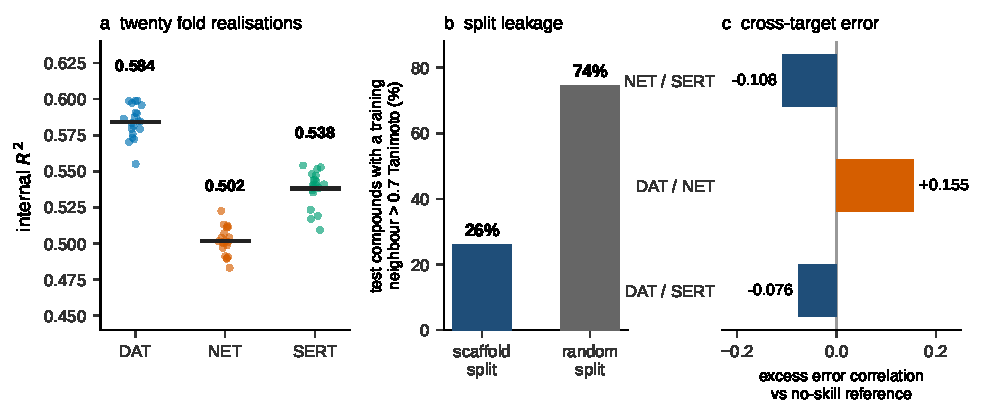
\includegraphics[width=\linewidth]{figures/fig2_internal.pdf}
\caption{Internal performance and split behaviour. (a) $R^2$ across twenty independent
scaffold-disjoint fold realisations; horizontal bars are means. Panel (a) is drawn from
the independent re-implementation of \S\,\ref{sec:reimplementation}, because that is the run
for which the per-realisation values were retained; its means are 0.584 / 0.502 / 0.538
against Table~\ref{tab:internal}'s 0.584 / 0.501 / 0.541, which are the originals and are
what every reported figure uses. (b) Percentage of test compounds having a training
neighbour above 0.7 Tanimoto under scaffold versus random splitting: scaffold splitting
reduces near-neighbour leakage but does not eliminate it. (c) Excess error correlation
between target pairs against a no-skill reference; positive values indicate shared model
bias. Error bars are SD across realisations.}
\label{fig:split}
\end{figure}

\subsection{The advance-specified external evaluation}

\begin{table}[tb]
\centering
\small
\caption{Advance-specified external evaluation. Bootstrap 95\% confidence intervals from
2000 resamples. n.s.\ = not significant.}
\label{tab:prereg}
\begin{tabular}{lcccc}
\toprule
Endpoint & Internal & External ($n=42$) & 95\% CI & $p$ \\
\midrule
\textbf{DAT/SERT ratio (primary)} & 0.564 & 0.114 & --- & 0.029 \\
pDAT  & 0.584 & 0.459 & $[0.209,0.690]$ & $<0.0001$ \\
pNET  & 0.501 & 0.015 & $[0.000,0.150]$ & 0.44 (n.s.) \\
pSERT & 0.541 & 0.058 & $[0.000,0.284]$ & 0.12 (n.s.) \\
\bottomrule
\end{tabular}
\end{table}

\begin{figure}[tb]
\centering
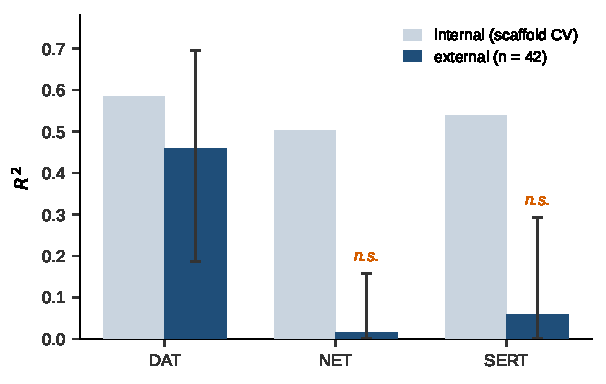
\includegraphics[width=\linewidth]{figures/fig3_external.pdf}
\caption{Advance-specified external test. Internal versus external $R^2$ with bootstrap
95\% confidence intervals; \textit{n.s.} marks correlations not distinguishable from zero.
The companion panel of post hoc sample-size calculations has been removed: observed-power
figures are a monotone transform of the $p$-value and add nothing the intervals do not
already carry.}
\label{fig:prereg}
\end{figure}

\textbf{The advance-specified primary endpoint failed its declared criterion}, falling
more than 0.20 below the internal estimate. At $n=42$, only DAT was adequately powered:
detecting correlations of the observed magnitude would require $n=15$ for DAT, $n=133$
for SERT and $n=515$ for NET. These are post hoc calculations based on observed
effects and largely restate the confidence intervals; the defensible statement is
that the available sample could not distinguish null from modest external
association at NET and SERT. Leakage does not explain the shortfall --- median
nearest-neighbour Tanimoto to training was 0.505, and no external compound exceeded
0.85.

\subsection{Decomposition of the shortfall}
\label{sec:decomp}

\begin{table}[tb]
\centering
\small
\caption{Matched-training decomposition. Internal cross-validated $R^2$ under training
sets matched to the external set on response range, chemotype, or both. The Baseline
column is a \emph{single} scaffold-CV realisation --- the one this experiment was run on
--- not the twenty-realisation mean of Table~\ref{tab:internal} (0.584 / 0.501 / 0.541).
The difference is within the realisation-to-realisation spread of $\pm0.013$ reported
there, and the comparison within this table is between columns computed on the same
realisation, which is what the decomposition requires.}
\label{tab:matched}
\begin{tabular}{lccccc}
\toprule
Target & Baseline & Range-matched & Chemotype-matched & Both & External \\
\midrule
pDAT  & 0.593 & 0.472 & 0.576 & 0.450 & 0.459 \\
pNET  & 0.511 & 0.248 & 0.458 & 0.195 & 0.015 \\
pSERT & 0.552 & 0.257 & 0.474 & 0.249 & 0.058 \\
\bottomrule
\end{tabular}
\end{table}

\begin{figure}[tb]
\centering
\small
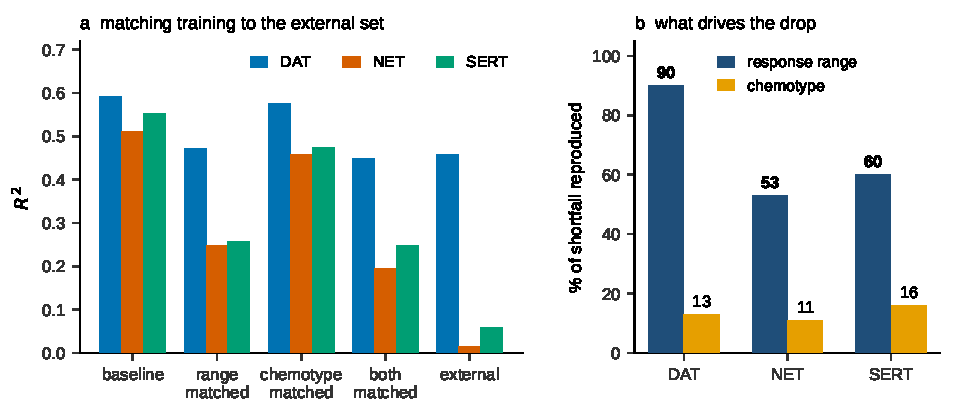
\includegraphics[width=\linewidth]{figures/fig6_decomposition.pdf}
\caption{Decomposition of the external shortfall. (a) $R^2$ under five independent matched-training conditions; these are separate analyses, not a sequence. For DAT the both-matched internal estimate (0.450) and the external result (0.459) coincide. (b) Percentage of the shortfall reproduced by each matching strategy.}
\label{fig:decomp}
\end{figure}

Range-restricted retraining --- a sensitivity analysis rather than a decomposition,
since it selects training data using the external response distribution ---
reproduces 90\%, 53\% and 60\% of the shortfall at DAT, NET and SERT
(bootstrap 95\% CI for NET $[51,73]$); chemotype matching reproduces only 13\%, 11\%
and 16\%.

\paragraph{Applicability domain.} Two complementary tests were applied. Mahalanobis
distance --- a multivariate measure accounting for covariance among descriptors,
not a per-descriptor percentile check --- placed the external compounds fully inside
the training distribution (holdout median 2.61 versus
training 2.73; 0\% beyond the training 95th percentile of 4.81). By contrast, 40\%,
33\% and 64\% of external compounds lay outside the training interquartile range at
DAT, NET and SERT. Similarity to the training set is an established predictor of per-compound error.
Sheridan tabulated it as a binned look-up populated by cross-validation at
model-build time, and validated prospectively on five Merck assays and more than
6000 compounds measured \emph{after} the models were built, finding the
cross-validated bin error a semiquantitative predictor of the prospective
error.\cite{Sheridan2012} That study also reports, on its own data, that bins built
on nearest-neighbour similarity alone cover a markedly smaller range of RMSE than
bins built on prediction variance or on the predicted value --- so similarity is the
weakest of the three parameters it examined. The present result, that
nearest-neighbour similarity contributes 2.2\% uniquely once response-range position
is in the model, is consistent with that ordering rather than at odds with it.
Nearest-neighbour ECFP4 Tanimoto to training had a median of 0.505 with no compound
above 0.85. The external compounds were therefore not extreme in the ten-descriptor
Mahalanobis space and were not close fingerprint near-duplicates, although scaffold
novelty was substantial and broader chemical novelty is excluded by neither test.
Descriptor-space inclusion is not chemical familiarity.

\begin{table}[tb]
\centering
\small
\caption{Error metrics across conditions. RMSE in log units.}
\label{tab:rmse}
\begin{tabular}{lcccc}
\toprule
Target & Baseline RMSE & Range-matched RMSE & External RMSE & Degradation \\
\midrule
pDAT  & 0.732 & 0.668 & 1.174 & $+76\%$ \\
pNET  & 0.807 & 0.680 & 0.848 & $+25\%$ \\
pSERT & 0.878 & 0.598 & 0.687 & $+15\%$ \\
\bottomrule
\end{tabular}
\end{table}

\begin{figure}[tb]
\centering
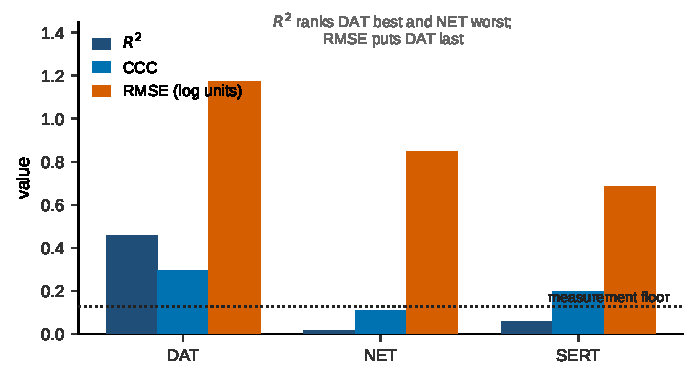
\includegraphics[width=\linewidth]{figures/fig7_metrics.pdf}
\caption{Metrics disagree on which target fared worst. $R^2$, concordance correlation coefficient and RMSE for the same external predictions. Dotted line is the aggregate measurement reproducibility floor (0.127 log units).}
\label{fig:metrics}
\end{figure}

On $R^2$, DAT appears best preserved and NET worst; on RMSE the order is close to
reversed, DAT scoring worst and SERT best. That $R^2$
depends on the spread of the test response, because its reference is the training-set mean,
was identified by Roy and co-workers, who proposed the $r_m^2$ family as a
remedy,\cite{Roy2009,Mitra2010} and has been restated with worked examples by
Alexander et al.\cite{Alexander2015} and by Martinez-Mayorga et
al.,\cite{MartinezMayorga2024} the latter showing a case in which the model with the
lowest absolute error also carries the lowest $R^2$ because its property range is
narrower.
Residual structure differs by target. DAT under-predicted throughout and worst at the
potent end (observed minus predicted $+0.982$ overall, $+1.443$ in the more potent half);
SERT over-predicted weak compounds ($-0.737$ in the weaker half). All three compressed
toward the training mean: regressing prediction on observation gives slopes of 0.379,
0.076 and 0.157, against 1 for no compression (Figure~\ref{fig:obspred}).

\paragraph{The matching comparison cannot be run in the other direction.}
Table~\ref{tab:matched} matches the \emph{training} set to the external set and asks how
much of the shortfall that reproduces. The natural complement is to match the
\emph{test} set: draw internal test sets with the external set's size, response
variance and nearest-neighbour similarity to training, and read off what the model would
have scored on a test set of that shape. That comparison is the one most readers will
want, and for most of these cells it does not exist.

For each external cell we asked where its response variance and its median
nearest-neighbour Tanimoto fall within the distribution of values attainable by
\emph{any} random internal subset of the same size, over 20\,000 draws
(Table~\ref{tab:reach}). For all nine cells at least one of the two lies outside that
distribution, and in every cell it is the similarity: the external sets' median
nearest-neighbour Tanimoto to training is 0.40--0.51, below the 1st percentile of what
random internal subsets of the matching size attain (0.48--0.55), and in most cells below
every one of the 20\,000 draws. Response variance is unreachable in four of the nine
cells in addition. Stalberga et al.'s SERT set has a response variance of 0.37 where
fewer than
1\% of internal subsets of 42 compounds fall below 1.07. No cell is matchable on both
constraints, so the comparison is nowhere defined.

This is not a technicality about sampling. A rejection sampler with a widening tolerance
--- the obvious implementation --- returns a band for all nine cells, because it widens
until something is accepted, and every band it returns is matched to nothing. We ran
four variants of this analysis during development and obtained three different headline
counts across them (six, six, five and four of nine ``inside the band'') before
establishing that no
cell admits the comparison at all. The attainability check, not the band, is the result.

This failure also has an established name. Requiring that a matched comparator exist for
every cell is the positivity, or common-support, condition of the matching and weighting
literature, and a sampler that returns an estimate where it is violated is the standard
cautionary case there.\cite{Westreich2010} We arrived at the check empirically and name it
here so that the general theory, and its diagnostics, carry over: what we are reporting is
that no internal subset lies in the support of the external sets' composition.

\paragraph{The one set that appeared matchable was the one that was contaminated.}
An earlier form of this analysis found three matchable cells, all three from the
PDSP/BindingDB set, and the reason it did is itself a result. That set was then filtered
for training overlap on the full InChIKey, which retains 30 of its 44 compounds. ECFP4 is
computed without stereochemistry, so thirteen of those 30 differed from a training
compound in stereochemistry alone and carried fingerprints identical to molecules the
model had been fitted on: nine recorded without stereodescriptors where the training
record specifies them, two resolved enantiomers of a racemate held flat in training, and
two --- the sertraline pair --- resolved differently on both sides. Their
nearest-neighbour similarity to training is 1.0 by construction, which lifted the set
median to 0.63 and into the attainable range. The model's mean absolute error on those
thirteen was 0.19--0.42 log units against 0.68--1.00 on the seventeen uncontaminated
compounds. Filtering on the InChIKey skeleton block removes them, and the set becomes as
unreachable as the other two. The attainability check selected, as the one external set
comparable to internal data, the one external set that in part \emph{was} internal data.

The two directions therefore answer different questions and give compatible answers. The
training-side manipulation succeeds because the training set \emph{contains} the
external response region --- one can restrict to it, and doing so reproduces 53--90\% of
the shortfall. The test-side manipulation fails because no random sample of the training
set \emph{resembles} the external sets --- they are not a narrow slice of the training
distribution but a deliberately selected region outside it, which is the quantitative
form of the coverage result in \S\,\ref{sec:cannot-evaluate}.

\begin{table}[tb]
\centering
\small
\caption{Whether a composition-matched internal comparator exists. Percentiles are the
position of the external value within the distribution attainable by random internal
subsets of the same size (20\,000 draws). ``---'' marks a value below the 1st percentile
of that distribution, for which no matched comparator can be constructed. Every cell
fails on similarity, and four also on variance; the sampler nonetheless returns a band
for all nine. All three sets are filtered for training overlap on the InChIKey skeleton
block; under the full-key filter used in an earlier draft the PDSP set retained 30
compounds, 13 of them fingerprint-identical to training compounds, and its similarity
median rose to 0.63 (69th percentile).}
\label{tab:reach}
\begin{tabular}{llrrcrc}
\toprule
Set & Target & $n$ & Variance & Percentile & NN Tanimoto & Percentile \\
\midrule
Stalberga 2026 & DAT  & 42 & 0.77 & --- & 0.51 & --- \\
               & NET  & 42 & 0.60 & --- & 0.51 & --- \\
               & SERT & 42 & 0.37 & --- & 0.51 & --- \\
PDSP/BindingDB & DAT  & 17 & 1.08 & 30th & 0.41 & --- \\
               & NET  & 17 & 1.42 & 65th & 0.41 & --- \\
               & SERT & 17 & 1.14 & 11th & 0.41 & --- \\
Cui 2026       & DAT  & 11 & 0.37 & --- & 0.41 & --- \\
               & NET  & 19 & 1.24 & 46th & 0.40 & --- \\
               & SERT & 18 & 0.77 & 1st  & 0.40 & --- \\
\bottomrule
\end{tabular}
\end{table}

\begin{figure}[tb]
\centering
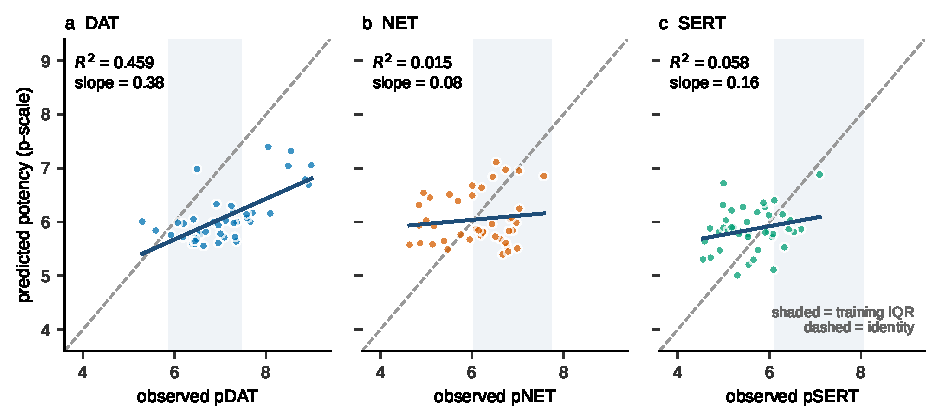
\includegraphics[width=\linewidth]{figures/fig4_obs_pred.pdf}
\caption{External predictions compress toward the training mean. Observed potency on the
abscissa and predicted on the ordinate, so the solid line is the regression of prediction
on observation and its slope is the annotated one; a slope of 1 would mean no
compression. Dashed line is identity, and the line is drawn only across the observed
range. Shaded band marks the training interquartile range.}
\label{fig:obspred}
\end{figure}

\begin{figure}[tb]
\centering
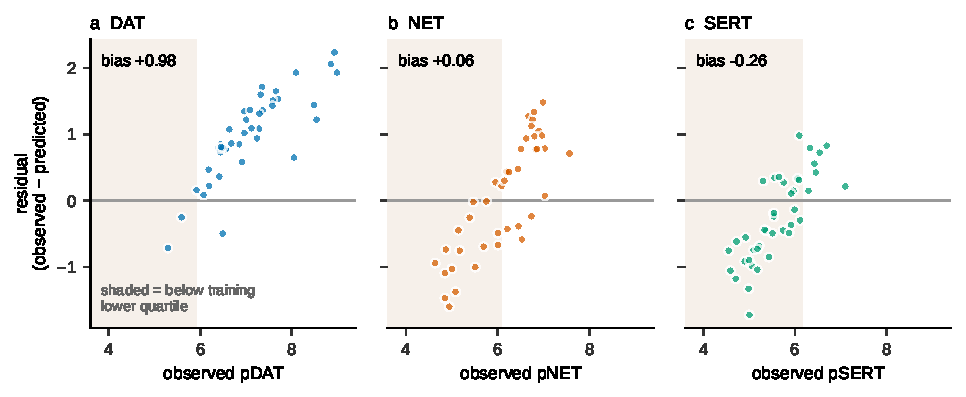
\includegraphics[width=\linewidth]{figures/fig5_residuals.pdf}
\caption{Residual structure differs by target. Shaded region marks values below the
training lower quartile. DAT under-predicts its most potent compounds; SERT
over-predicts weak ones.}
\label{fig:resid}
\end{figure}

\begin{figure}[tb]
\centering
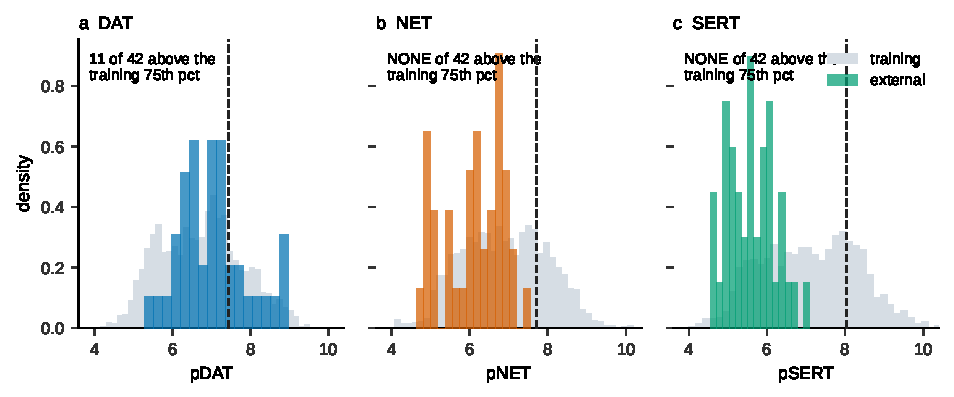
\includegraphics[width=\linewidth]{figures/fig10_coverage.pdf}
\caption{The advance-specified external set contains no potent NET or SERT ligands. Grey is
the uncensored training distribution and the dashed line its 75th percentile; the
coloured histogram is the 42 external compounds. Eleven clear the line at DAT and none
at NET or SERT. The two sets assembled afterwards do reach above it
(Figure~\ref{fig:newsets}).}
\label{fig:coverage}
\end{figure}

\subsection{Assay modality (exploratory)}
\label{sec:assay-modality}

\begin{table}[tb]
\centering
\small
\caption{Binding-versus-functional offsets. Positive values indicate higher potency in
the functional assay.}
\label{tab:assay}
\begin{tabular}{lcrc}
\toprule
Target & $n$ & Median offset & SD \\
\midrule
DAT  & 112 & $-0.168$ & 0.529 \\
NET  &  97 & $\mathbf{+0.440}$ & 0.658 \\
SERT &  77 & $-0.083$ & 0.497 \\
\bottomrule
\end{tabular}
\end{table}

\begin{figure}[tb]
\centering
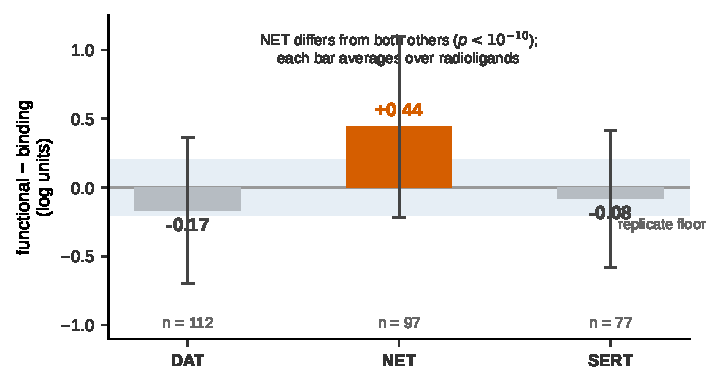
\includegraphics[width=\linewidth]{figures/fig9_assay.pdf}
\caption{The binding-versus-functional offset is positive at NET and not at DAT or SERT,
on the frozen set. Median difference between functional and binding potency for compounds
measured both ways, with SD; shaded band is the replicate reproducibility floor. The
robust contrast is NET against the other two. DAT and SERT are not distinguishable from
one another here ($p=0.39$) but are on the independent re-retrieval ($p=0.005$), so no
claim of DAT--SERT equality should be read from this figure. Each bar also averages over
radioligands, which Table~\ref{tab:radioligand} separates.}
\label{fig:assay}
\end{figure}

Kruskal--Wallis $p=2.7\times10^{-11}$. Cross-assay dispersion is 2.6--3.4 times the
replicate reproducibility floor at every target, making assay modality a larger error
source than measurement error. Applying the measured NET offset as a constant correction did \emph{not} improve
external fit (RMSE $0.848\rightarrow0.925$). The dispersion of the offset (SD 0.658)
is larger than its median (0.440), so the discrepancy is not a fixed additive shift
but varies by compound and, plausibly, by assay conditions such as substrate
concentration and incubation time, which differ between the contributing studies. A
correction that transfers between datasets would need to be conditioned on those
factors rather than applied as a constant.

\subsection{The NET offset replicates and is not carried by one chemotype}
\label{sec:chemotype}

Two questions follow from \S\,\ref{sec:assay-modality}. Does the offset survive a different retrieval of
the source database, and is it a property of the transporter or of a single
chemotype? Both were addressed with the independent re-retrieval described in
\S\,\ref{sec:rederivation}.

\textbf{Replication.} The NET offset reproduces at $+0.540$ (95\% CI $+0.390$ to
$+0.670$; $n=81$; Wilcoxon $p=1.2\times10^{-8}$), slightly larger than the frozen
estimate of $+0.440$. DAT gives $-0.280$ ($[-0.380,-0.170]$, $n=89$) and SERT
$-0.080$ ($[-0.180,+0.000]$, $n=71$); Kruskal--Wallis across the three targets
$p=2.7\times10^{-16}$. The NET-versus-other-targets contrast therefore holds across
sixteen months of database revision and an independently written curation script.

\textbf{Chemotype stratification.} Every stratum of the re-retrieved NET set with
$n\geq5$ shows a positive median offset (Table~\ref{tab:chemotype},
Figure~\ref{fig:chemotype}): five of five Butina clusters at 0.6 Tanimoto, and four
of four Bemis--Murcko scaffold strata, the latter spanning $+0.31$ to $+1.07$.
Deleting the largest cluster outright --- the 25 pyrrolidinophenones --- leaves the
pooled offset at $+0.390$; no leave-one-stratum-out deletion moves it by more than
0.15 or changes its sign. No single chemotype carries the effect. That is a statement
about chemotypes as the manuscript's own strata define them; \S\,\ref{sec:radioligand-results}
shows that the radioligand strata, which are close to disjoint in chemistry, do not behave
alike, and that the chemotype strata used here do not settle the question.

\textbf{But the magnitude is chemotype-dependent.} The offset differs significantly
across strata (Kruskal--Wallis, $p<0.001$), spanning roughly threefold from $+0.31$
to $+0.99$, and is largest in the pyrrolidinophenone ($\alpha$-pyrrolidinovalerophenone-type)
cathinones --- the chemotype of greatest interest for novel psychoactive substance
profiling. The pooled figure is thus an average over a heterogeneous set. This is
consistent with, and supplies a mechanism for, the failure of the constant correction
reported in \S\,3.5: a transferable correction would have to be chemotype-resolved,
and the per-stratum samples available here ($n=5$ to $n=25$) are too small to
estimate one.

\begin{table}[tb]
\centering
\small
\caption{Chemotype stratification of the NET binding-versus-functional offset on the
independent re-retrieval ($n=81$). Strata are Butina clusters of ECFP4 fingerprints
at 0.6 Tanimoto. Stratum labels are descriptive readings of the Bemis--Murcko
scaffold of each cluster centroid; the exact scaffold SMILES are in the deposited
repository. Confidence intervals are percentile bootstrap (4000 resamples). Every
stratum is positive.}
\label{tab:chemotype}
\begin{tabular}{lrrc}
\toprule
Chemotype stratum & $n$ & Median offset & 95\% CI \\
\midrule
Pyrrolidinophenones ($\alpha$-PVP-type) & 25 & $+0.99$ & $[+0.69,+1.10]$ \\
Fused imidazoline tricyclics              & 10 & $+0.86$ & $[+0.38,+1.38]$ \\
Naphthyl norbornanes                      &  5 & $+0.64$ & $[+0.39,+0.78]$ \\
Benzhydryl ether amines (GBR-type)        &  5 & $+0.40$ & $[-0.15,+0.45]$ \\
3-Aryltropanes                            & 17 & $+0.31$ & $[-0.17,+0.39]$ \\
\midrule
All compounds                             & 81 & $\mathbf{+0.54}$ & $[+0.39,+0.67]$ \\
\bottomrule
\end{tabular}
\end{table}

\begin{figure}[tb]
\centering
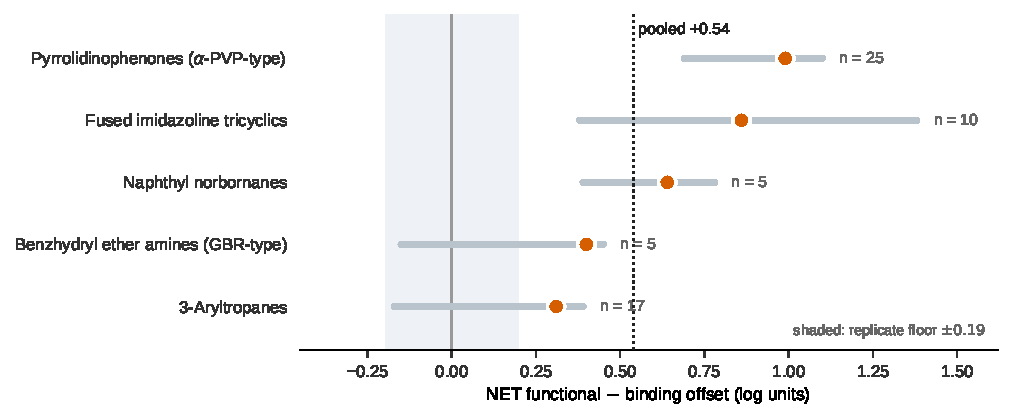
\includegraphics[width=\linewidth]{figures/fig11_chemotype.pdf}
\caption{The NET binding-versus-functional offset within each chemotype, on the
independent re-retrieval. Every stratum is positive; the magnitude varies roughly
threefold. Dotted line marks the pooled estimate. Bars are 95\% percentile bootstrap
intervals.}
\label{fig:chemotype}
\end{figure}

\paragraph{One discrepancy between retrievals.} In the frozen analysis the DAT and
SERT offsets were not distinguishable from one another ($p=0.39$). In the
re-retrieval they are ($-0.280$ versus $-0.080$; Mann--Whitney $p=0.005$), driven by
a more negative DAT estimate on a different compound set. We therefore claim that the
offset is specific to NET among the three targets --- a contrast robust to retrieval
and curation --- and \emph{not} that DAT and SERT behave identically. The caption of
Figure~\ref{fig:assay} should be read in that narrower sense.

\subsection{The offset survives within single papers and is not the releaser effect}
\label{sec:within-doc}
\label{sec:confounds-results}

\paragraph{It is not a between-laboratory artefact.} Of the 81 NET paired compounds,
75 have both their binding $K_i$ and their functional IC$_{50}$ reported in the
\emph{same} paper. Restricted to those within-document pairs the offset is
$+0.550$ (95\% CI $[+0.400,+0.690]$; Wilcoxon $p=1.0\times10^{-9}$), indistinguishable
from the $+0.540$ obtained by pooling across documents. Five documents contribute, from
five different laboratories and spanning 1999--2007
(Figure~\ref{fig:within}): Choi et al.\ 1999 \cite{Choi1999} ($n=10$, $+0.15$),
Houlihan et al.\ 2002 \cite{Houlihan2002} ($n=13$, $+1.12$), Axford et
al.\ 2003 \cite{Axford2003} ($n=8$, $+0.47$), Meltzer et al.\ 2006 \cite{Meltzer2006}
($n=29$, $+0.99$) and Gong et al.\ 2007 \cite{Gong2007} ($n=17$, $+0.31$). Every one is
positive. Dropping the largest contributor leaves a median of $+0.390$ across the
remaining four documents and 48 compounds. Because the two values within a paper are produced by one group on one
compound batch, this comparison removes between-laboratory calibration differences
entirely, and the offset is unchanged.

\paragraph{The same test at DAT and SERT separates NET from the other two.} Repeating
the analysis on the DAT and SERT paired sets gives $-0.280$ on 86 within-document pairs
(95\% CI $[-0.380,-0.155]$) and $-0.090$ on 66 (95\% CI $[-0.220,-0.010]$), against
$+0.550$ at NET; Kruskal--Wallis across the three $H=77.6$, $p=1.4\times10^{-17}$. Adding
the Eshleman blockers described below as a sixth source --- merging the two compounds
common to both, cocaine and mazindol, so that no compound is counted twice --- gives
pooled estimates of $-0.180$ at DAT ($n=100$, 95\% CI $[-0.300,-0.070]$), $\mathbf{+0.600}$
at NET ($n=89$, $[+0.470,+0.748]$, Wilcoxon $p=2.9\times10^{-12}$) and $-0.048$ at SERT
($n=80$, $[-0.130,+0.110]$, $p=0.38$); Kruskal--Wallis $H=91.5$,
$p=1.3\times10^{-20}$. Only NET is distinguishable from zero in the positive direction,
and SERT is not distinguishable from zero at all.

The per-source pattern is the more informative one. At NET all six sources agree in
sign; at DAT and SERT they do not (DAT $-0.51$ to $+0.28$, SERT $-0.34$ to $+0.19$), so
what is a consistent directional offset at NET is scatter about zero at the other two
transporters (Figure~\ref{fig:within}). This is the same NET-specific contrast reported
in \S\,\ref{sec:chemotype} and Table~\ref{tab:assay}, now established without any
between-study comparison.

\paragraph{Robustness of the NET result.} Four distribution-free checks, each aimed at a
different objection. (i) The direction is near-unanimous at the compound level rather than
carried by a tail: 64 of 75 within-document NET pairs are positive (85.3\%, exact 95\% CI
$[75.3,92.4]$, sign test $p=3.1\times10^{-10}$), against 24 of 86 at DAT and 24 of 66 at
SERT. (ii) A sign-flip permutation test --- the exact null for a paired design, in which
the two modality labels are exchangeable within a compound --- gives an observed median
of $+0.550$ against a null range of $[-0.450,+0.400]$ over 20\,000 relabellings
($p<5\times10^{-5}$); the corresponding SERT value falls inside its null ($p=0.21$).
(iii) Taking the \emph{source} rather than the compound as the unit of analysis, 6 of 6
sources are positive at NET (sign test $p=0.031$, the minimum attainable at $n=6$) against
2 of 6 at DAT and 2 of 5 at SERT. (iv) The separation between targets is large by
distribution-free effect size: Cliff's $\delta=+0.729$ for NET against DAT and $+0.665$
against SERT. Leave-one-document-out leaves $+0.390$ at worst, removing Meltzer et al.'s
29 compounds.

\paragraph{It is not the releaser-versus-blocker distinction.} All 81 paired compounds
classify as uptake blockers. None carries a release or efflux assay record in ChEMBL
(0 of 785 retrieved DAT/NET/SERT records), and none matches the substrate-type releaser
pharmacophore: the set is dominated by $\alpha$-pyrrolidinophenones, mazindol-type
isoindoles, 3$\beta$-aryltropanes and benzhydryl ethers, with a median molecular weight
of 303\,Da and a single compound below 230\,Da. Amphetamine-type releasers are absent
by construction, because paired binding-and-functional measurements at NET come almost
entirely from medicinal-chemistry uptake-inhibitor series. Two internal controls
confirm the scale: cocaine gives $+0.78$ and mazindol $+0.50$ here, against the $7.0$-
and $5.0$-fold NET ratios ($+0.85$ and $+0.70$ log units) reported for the same two
compounds by Eshleman et al.\cite{Eshleman2017} The offset is therefore a property of
blockers, measured within blockers, and the releaser mechanism cannot account for it.

\paragraph{Half of the paired offset is the value type, not the assay format.} The
$+0.550$ above compares binding $K_i$ with functional IC$_{50}$, and in ChEMBL those
two attributes travel together: binding records are predominantly $K_i$ and functional
records predominantly IC$_{50}$. The comparison therefore moves assay format and value
type at once, and Cheng--Prusoff alone predicts a difference between $K_i$ and
IC$_{50}$.\cite{Kalliokoski2013} With modality labelled from assay text rather than
from \texttt{standard\_type} (\S\,\ref{sec:modality-labelling}) the off-diagonal cells
are populated --- 3018 binding IC$_{50}$ and 1336 functional $K_i$ records --- and the
two can be estimated in one model.

Fitted with compound-within-document fixed effects and document-clustered standard
errors across 1169 informative records from 49 documents and 512 compounds, the
assay-format component at NET is $\mathbf{+0.261}$ (95\% CI $[+0.06,+0.46]$,
$p=0.010$) and the $K_i$-versus-IC$_{50}$ component is indistinguishable from zero
($-0.047$, $p=0.52$). Both components are null at DAT ($+0.003$, $p=0.98$; value type
$+0.107$, $p=0.088$) and SERT ($+0.036$, $p=0.84$; value type $+0.184$, $p=0.20$), so
the NET specificity reported above survives the decomposition while its magnitude
halves (Table~\ref{tab:twobytwo}).

The two estimates are not in conflict; the larger one is the sum of both components.
Applied to the five paired documents alone, the same model gives $+0.578$ for format
when the value-type term is omitted --- recovering the $+0.550$ reported above --- and
$+0.289$ when it is included, which is within confidence of the corpus-wide $+0.261$.
The paired estimate is the clean within-series demonstration; the fixed-effects
estimate is the one to generalise from, and it rests on roughly eight times as many
documents.

\paragraph{The format effect survives among blockers alone, at corpus scale.} The
structural classification of \S\,\ref{sec:twobytwo} assigns 42 of 5796 compounds as
substrate-type and 5754 as blockers. Restricting the model to blockers leaves the NET
format effect at $+0.238$ (95\% CI $[+0.04,+0.43]$, $p=0.018$; 1095 records, 49
documents, 487 compounds), and substrate-type compounds are 1.9\% of the NET
informative records, so they cannot be carrying it. The substrate stratum itself shows
a larger offset ($+1.28$), directionally consistent with the $K_\mathrm{m}\neq
K_\mathrm{D}$ account \cite{Schomig1988} and with the Eshleman releaser values above,
but it rests on three documents and no interval is quoted for it.

Robustness: leave-one-document-out leaves the corpus-wide NET estimate between $+0.227$
and $+0.331$ and significant in 272 of 272 fits; moving the \texttt{conflict} class
into either modality leaves it at $+0.261$, since only 40 of those 810 records are NET
and none falls in an informative group; document fixed effects in place of
compound-within-document effects give $+0.253$ ($p=0.032$).

\paragraph{The cluster count.} Forty-nine clusters is few enough that CR0 cluster-robust
variance over-rejects, so the interval above is not the one to quote. A wild cluster
bootstrap-$t$ with Rademacher weights and 9999 replications, clustered on document and
imposing the null, widens the NET format effect to $[+0.024,+0.486]$ with $p=0.028$
against the CR0 $[+0.062,+0.460]$ and $p=0.010$. The correction matters and the effect
survives it. The value-type component is null either way ($[-0.17,+0.07]$, $p=0.53$). Intervals
elsewhere in this paper are CR0 unless stated, including in
Table~\ref{tab:radioligand}, where quoting ten bootstrap intervals would obscure the
comparison between strata; the bootstrap interval is given in the text for each estimate
the argument rests on, and is always the wider of the two.

\begin{table}[tb]
\centering
\caption{Assay format and value type, estimated jointly. Compound-within-document fixed
effects, standard errors clustered on document. Positive values mean the first-named
condition reads more potent. The format effect is NET-specific; the value-type effect
is not, and at NET it is absent.}
\label{tab:twobytwo}
\begin{tabular}{lrrrll}
\toprule
Target & Records & Documents & Compounds & Functional $-$ binding & p$K_i$ $-$ pIC$_{50}$ \\
\midrule
DAT  &  932 & 49 & 388 & $+0.003$ $[-0.16,+0.17]$ & $+0.107$ $[-0.02,+0.23]$ \\
NET  & 1169 & 49 & 512 & $\mathbf{+0.261}$ $[+0.06,+0.46]$ & $-0.047$ $[-0.19,+0.09]$ \\
SERT &  939 & 47 & 380 & $+0.036$ $[-0.32,+0.39]$ & $+0.184$ $[-0.10,+0.46]$ \\
\midrule
\multicolumn{4}{l}{NET, uptake blockers only} & $+0.238$ $[+0.04,+0.43]$ & \\
\bottomrule
\end{tabular}
\end{table}

\subsection{The offset is a property of the assay cell, not of the assay format}
\label{sec:radioligand-results}

Everything above treats the binding side of the comparison as one thing. It is not. The
assay descriptions name the radioligand (\S\,\ref{sec:radioligand}), and splitting on it
changes the reading of the result.

\paragraph{At NET the effect is confined to one radioligand.} Refitting the model of
Table~\ref{tab:twobytwo} inside each radioligand stratum --- still compound-within-document
effects, still document-clustered --- gives a format effect of $\mathbf{+0.507}$ (CR0 95\% CI
$[+0.34,+0.68]$, $p=3\times10^{-9}$; wild cluster bootstrap-$t$ $[+0.20,+0.82]$,
$p=0.005$, and the bootstrap is the interval to read, on 17 clusters) in the 17 documents using
[$^{125}$I]RTI-55, and $\mathbf{+0.038}$ ($[-0.18,+0.26]$, $p=0.73$) in the 21 using
[$^{3}$H]nisoxetine (Table~\ref{tab:radioligand}). The pooled $+0.261$ is an average of a
large effect and a null; the nisoxetine interval is centred near zero and only barely
reaches the pooled estimate.

The within-document medians agree, which matters because that contrast removes
between-laboratory calibration by construction: $+0.530$ over 175 pairs in 12 RTI-55
documents against $-0.115$ over 146 pairs in 10 nisoxetine documents (Mann--Whitney
$p=5.5\times10^{-16}$). Eleven of the twelve RTI-55 documents are positive; the ten
nisoxetine documents are six negative and four positive, centred near zero. Four of the
five papers behind the $+0.550$ paired estimate of \S\,\ref{sec:within-doc} use
[$^{125}$I]RTI-55.

\paragraph{It is not simply that RTI-55 reads low.} Within the RTI-55 stratum NET remains
the outlier, at $+0.507$ against $+0.183$ at DAT and $-0.031$ at SERT. And within the
target-specific ligands the spread is wider still: $-0.308$ for [$^{3}$H]WIN\,35,428 at
DAT and $-1.044$ for [$^{3}$H]paroxetine at SERT. The offset is therefore a property of
the assay cell --- here indexed by target and radioligand, which is the stratification the
data support and not a claim about which of the two is operative --- ranging over 1.5 log
units across the binding assays in this corpus, and each per-target estimate is a composition-weighted average over whichever
radioligands happen to dominate that target's literature. NET looks special in pooled data
because NET is where [$^{125}$I]RTI-55 --- the cell with the largest positive offset --- is
most used.

\paragraph{What this does and does not establish.} Radioligand is confounded with document
and nearly with chemotype, and the data cannot separate them. Only four NET documents use
more than one binding radioligand and none has enough two-ligand overlap to give a
within-document radioligand contrast. The two NET strata share 5 compounds out of 174 and
163, their median molecular weights are 285 and 365, and their median cross-stratum
nearest-neighbour Tanimoto is 0.28 --- the RTI-55 stratum is stimulant-like and the
nisoxetine stratum is medicinal-chemistry NET series. What the stratification establishes
is that the pooled estimate is an average over heterogeneous assay cells, not that the
radioligand rather than the chemistry is the operative variable. A mis-specified $K_D$ in
the Cheng--Prusoff conversion for RTI-55 at NET would produce exactly a constant shift in
every $K_i$ from that assay at one target, which fits the observed pattern, but this
corpus cannot confirm it. Resolving it needs an experiment: the same compounds at NET by
both radioligands in one laboratory.

\begin{table}[tb]
\centering
\small
\caption{The binding-versus-functional offset by binding radioligand. Compound-within-document
fixed effects, document-clustered standard errors, as in Table~\ref{tab:twobytwo}; a
document is assigned to the radioligand it uses for the most binding records. The
\emph{all} rows are Table~\ref{tab:twobytwo} repeated for comparison. The format effect
is not a property of the format: it spans 1.5 log units across binding assays.}
\label{tab:radioligand}
\begin{tabular}{llrrr}
\toprule
Target & Binding radioligand & Documents & Records & Functional $-$ binding \\
\midrule
DAT  & all                      & 49 &  932 & $+0.003$ $[-0.16,+0.17]$ \\
     & [$^{125}$I]RTI-55        & 20 &  634 & $+0.183$ $[-0.01,+0.38]$ \\
     & [$^{3}$H]WIN\,35,428     & 12 &  148 & $-0.308$ $[-0.49,-0.13]$ \\
\midrule
NET  & all                      & 49 & 1169 & $\mathbf{+0.261}$ $[+0.06,+0.46]$ \\
     & [$^{125}$I]RTI-55        & 17 &  654 & $\mathbf{+0.507}$ $[+0.34,+0.68]$ \\
     & [$^{3}$H]nisoxetine      & 21 &  411 & $\mathbf{+0.038}$ $[-0.18,+0.26]$ \\
\midrule
SERT & all                      & 47 &  939 & $+0.036$ $[-0.32,+0.39]$ \\
     & [$^{125}$I]RTI-55        & 18 &  417 & $-0.031$ $[-0.22,+0.16]$ \\
     & [$^{3}$H]citalopram      &  9 &   80 & $-0.055$ $[-0.21,+0.10]$ \\
     & [$^{3}$H]paroxetine      &  6 &  274 & $-1.044$ $[-1.39,-0.70]$ \\
\bottomrule
\end{tabular}
\end{table}

\paragraph{The offset is real and not exploitable.} Separating the two modalities does
not improve prediction. Trained and cross-validated on modality-specific labels, models
predicting modality-specific values gain $+0.002$ $r^{2}$ on average over models trained
on pooled labels (range $-0.010$ to $+0.016$ across six target $\times$ modality cells).
Externally, where each test set was measured in one modality --- Stalberga et al.\ and
Cui et al.\ by functional uptake, the PDSP/BindingDB panel by radioligand binding ---
scoring with the matching-modality model is \emph{worse} than scoring with the pooled
model by $-0.067$ $r^{2}$ (better in 2 of 9 cells, Wilcoxon $p=0.25$). A size-matched
control attributes most of that to data quantity rather than to modality: refitting the
pooled model on a random subset the size of the modality model costs $-0.050$ on its
own, leaving $-0.017$ attributable to the separation itself.

This closes the loop on the constant correction reported in
\S\,\ref{sec:assay-modality}, which also worsened external fit. The offset at NET is
measurable, replicable, specific and mechanistically interpretable, and none of the
three obvious ways of acting on it --- correcting by it, training separately on it, or
selecting the matching modality at test time --- recovers any accuracy. A difference
that is detectable in aggregate need not be large enough, relative to the spread around
it (SD 0.658 against a median of 0.440), to carry information about any individual
compound.

\paragraph{An independent within-document replication, with the classes separated.}
Eshleman et al.\cite{Eshleman2017} is itself a single-laboratory source reporting both
modalities on the same compounds, and it classifies each compound as blocker or
substrate by a [$^3$H]neurotransmitter \emph{release} assay --- a criterion that does
not use the ratio under test. Their Table~2 therefore permits the cleanest available
version of this comparison. Across their 16 uptake blockers the offset is $+0.752$ at
NET (95\% CI $[+0.699,+0.914]$) against $+0.279$ at DAT and $+0.176$ at SERT
(Kruskal--Wallis $H=26.0$, $p=2.2\times10^{-6}$) --- the same NET-specific excess, in an
independent dataset, among compounds independently confirmed not to be substrates.
Their 15 substrate-type releasers sit one to two log units higher at every transporter
($+1.36$, $+2.14$, $+1.54$ at DAT, NET, SERT), which is why the class has to be excluded
before the modality effect can be read, and why a ratio-based classification of the
present paired set would have been circular. The elevation is expected and is not a
competing measurement of the same quantity: substrate affinity is low by design, because
a transported compound must release on the far side of the membrane, while a substrate
suppresses \emph{net} uptake not only by competing for the site but by consuming
transport cycles, eroding the sodium gradient and driving reverse transport --- a large
$K_i$ and a small IC$_{50}$ from the same molecule. Notably the shift is close to uniform
across the three transporters ($+1.08$, $+1.39$, $+1.36$ relative to the same paper's
blockers), so the NET-specific excess is approximately additive on top of it ($+0.53$
within blockers, $+0.69$ within releasers) rather than being produced by it.

\begin{figure}[tb]
\centering
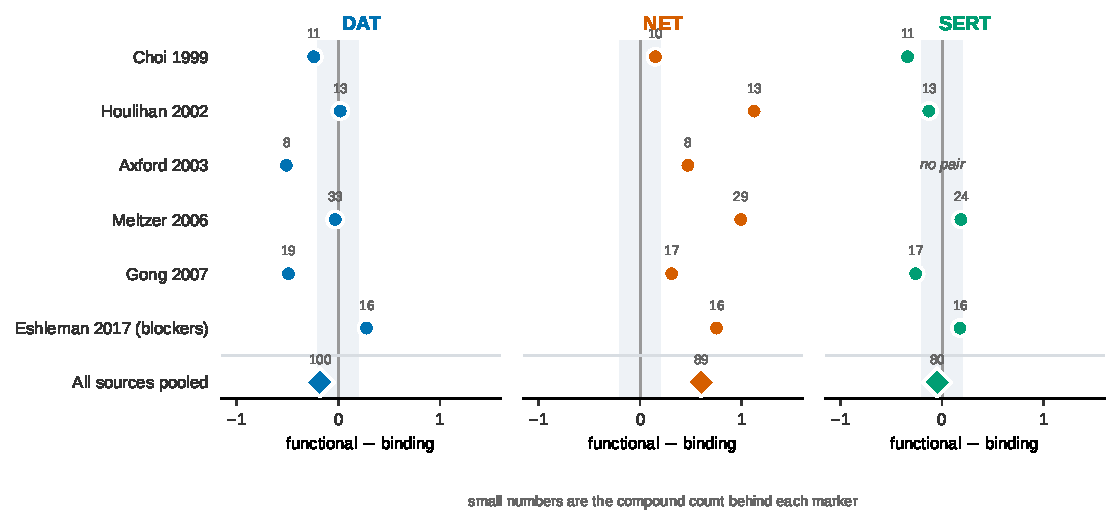
\includegraphics[width=\linewidth]{figures/fig12_within_document.pdf}
\caption{The binding-versus-functional offset measured within single papers, where both
modalities come from one laboratory on one compound series, so no between-study
calibration difference can contribute. Each of the first six rows is one source; the
final row pools them, taking one value per compound so that cocaine and mazindol, which
appear in both the Eshleman panel and the ChEMBL series, are counted once. Markers are
medians and bars 95\% percentile bootstrap intervals. At NET every source agrees in sign;
at DAT and SERT they do not. Small numbers are the compound count behind each marker.
Axford et al.\ contributed no SERT pair. The Eshleman row is their uptake blockers only,
classified by their release assay; their substrate-type releasers are excluded and are
reported in the text.}
\label{fig:within}
\end{figure}

\subsection{Extended external evaluation (exploratory)}
\label{sec:extended}

The extended set comprises 114 compounds across 31 scaffolds from four laboratories,
with response range restored to near-training levels (log-ratio SD 1.39 versus 1.41).
Document-level leakage probes returned zero DAT/NET/SERT activities from any
contributing source. The log-ratio is modelled \emph{directly}, as one regressor
trained on the log-ratio, rather than differenced from the two per-target models; the
differenced route is less conservative ($R^2=0.352$ on the same compounds). The pooled
statistic is computed on the 107 compounds from the three Basel and Link\"oping
sources, the seven Eshleman compounds being reported separately by source in
Table~\ref{tab:source} rather than pooled. DAT/SERT log-ratio prediction:
$R^2=0.183$, 95\% CI $[0.058,0.336]$, $r=+0.427$, $p=4.4\times10^{-6}$, RMSE 1.335,
CCC 0.304.

\begin{table}[tb]
\centering
\footnotesize
\setlength{\tabcolsep}{4pt}
\caption{Extended external performance by source. Scaf.\ = distinct Murcko scaffolds;
NN = nearest-neighbour Tanimoto to training. Confidence intervals are percentile
bootstrap (2000 resamples) and overlap substantially across sources. The OHSU row
($n=7$, 3 scaffolds) is reported for completeness only: its $R^2$ is not
interpretable at that sample size, as its simultaneously highest $R^2$ and worst
RMSE illustrate.}
\label{tab:source}
\begin{tabular}{lrrrlrrrr}
\toprule
Source & $n$ & Scaf. & SD($y$) & $R^2$ (95\% CI) & RMSE & MAE & Bias & Med NN \\
\midrule
Luethi \& Liechti 2020 (Basel) & 39 & 12 & 1.33 & 0.412 [0.143, 0.649] & 1.065 & 0.842 & $-0.309$ & 0.500 \\
Basel primary studies & 26 & 11 & 1.15 & 0.357 [0.084, 0.655] & 1.068 & 0.815 & $+0.565$ & 0.444 \\
Stalberga et al.\ 2026 (Link\"oping) & 42 & 14 & 0.97 & 0.114 [0.001, 0.420] & 1.668 & 1.463 & $+1.383$ & 0.505 \\
Eshleman et al.\ 2017 (OHSU)$^{a}$ & 7 & 3 & 0.78 & 0.773 [0.446, 0.991] & 1.687 & 1.651 & $+1.651$ & 0.667 \\
\bottomrule
\end{tabular}
\end{table}

Two features of Table~\ref{tab:source} caution against reading it as a laboratory
effect. The sources differ significantly in chemical novelty (Kruskal--Wallis,
$H=13.95$, $p=0.003$), so they cannot be treated as comparably novel. And the OHSU set
has the highest $R^2$ (0.773) together with the worst RMSE (1.687) and largest bias
($+1.651$) --- at $n=7$, $R^2$ is not interpretable.

\begin{table}[tb]
\centering
\small
\caption{Variance decomposition of external error. Unique contribution is the
semi-partial $R^2$ of an ordinary least-squares model of absolute prediction error:
the drop in model $R^2$ when that block alone is removed. Confidence intervals are
percentile bootstrap over external compounds (2000 resamples).}
\label{tab:vardecomp}
\begin{tabular}{lccc}
\toprule
Predictor block & $R^2$ alone & \textbf{Unique} & 95\% CI \\
\midrule
\textbf{Response-range position} & 0.444 & \textbf{0.308} & [0.187, 0.416] \\
Chemical similarity              & 0.024 & 0.022 & [0.000, 0.071] \\
Source identity                  & 0.178 & 0.021 & [0.005, 0.077] \\
\midrule
All three together               & \textbf{0.495} & --- & [0.374, 0.639] \\
\bottomrule
\end{tabular}
\end{table}

\begin{figure}[tb]
\centering
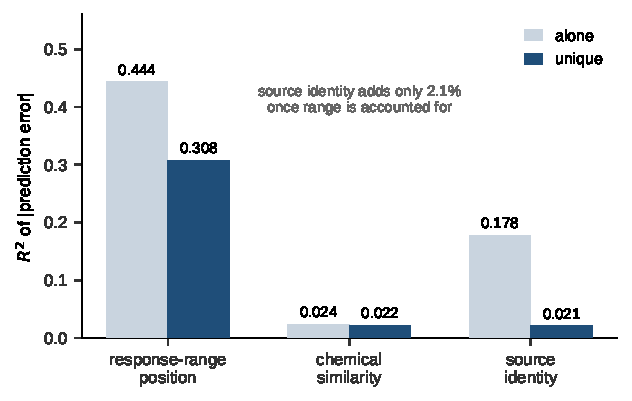
\includegraphics[width=0.62\linewidth]{figures/fig8_source.pdf}
\caption{An outcome-conditioned error diagnostic on the extended external set
($n=114$). Unique contributions from a regression of absolute prediction error on
response-range position, chemical similarity and source identity; ``alone'' is each
block's own $R^2$ and ``unique'' the drop in model $R^2$ when that block is removed.
The figure is reported as a caution rather than as a result: the analysis is
outcome-conditioned and largely reproduces prediction shrinkage
(Table~\ref{tab:circular}).}
\label{fig:vardecomp}
\end{figure}

\textbf{This diagnostic is largely circular.} The failure has a name outside
cheminformatics: it is endogenous selection bias from conditioning on a quantity that is
itself a function of the outcome, the general statement of which is the causal-inference
literature on collider and post-outcome conditioning.\cite{Elwert2014} Response-range
position is computed from the observed external value, and absolute error is computed from
the same value. A regularised model shrinks predictions toward the training mean, so error is
mechanically larger for compounds far from that mean. Here predictions had SD 0.717
against observations at 1.382, and an observation's distance beyond the training
interquartile range correlated with its distance from the training mean at
$r=0.983$.

Three comparisons establish that the apparent effect is mechanical
(Table~\ref{tab:circular}). Regressing absolute error on range position gives
$R^2=0.444$. Substituting the naive shrinkage predictor --- distance from the
training mean, which involves no notion of range --- reproduces it at $R^2=0.448$.
The only form available before the external outcome is known, using the distance of
the \emph{prediction} from the training mean, collapses to $R^2=0.001$. A model
predicting the training mean for every compound would give $R^2=0.966$ by
construction.

\begin{table}[tb]
\centering
\small
\caption{An outcome-conditioned error diagnostic is largely circular. Each row
regresses absolute external error on a single predictor. The quantity available
before the external outcome is known (third row) carries essentially no information.}
\label{tab:circular}
\begin{tabular}{lc}
\toprule
Predictor of $|$external error$|$ & $R^2$ \\
\midrule
Response-range position (outcome-conditioned) & 0.444 \\
Distance from training mean (shrinkage null) & 0.448 \\
Distance of \emph{prediction} from training mean & \textbf{0.001} \\
\midrule
Mechanical ceiling (model predicts training mean) & 0.966 \\
\bottomrule
\end{tabular}
\end{table}

We therefore make no causal claim about the determinants of external error. What the
analysis establishes is narrower and still useful: external error here is dominated
by prediction shrinkage outside the training response region, a property of
regularised regression rather than a discovery about chemical generalisation.
Investigators reporting similar decompositions should check them against a shrinkage
null before interpretation. Source identity and chemical similarity contribute little
unique variance conditional on the response-range measure included here; because the two
predictors are strongly confounded by construction, that is a statement about this
regression and not evidence that laboratory effects are unimportant in general.

\paragraph{What to use instead.} Ending on a caution leaves the practical question open,
and it has an answer this paper did not supply. The quantity the failed diagnostic was
reaching for --- a per-compound estimate of how far a prediction can be trusted, available
\emph{before} the outcome is known --- is what conformal prediction provides, with a
validity guarantee under exchangeability and without any conditioning on the observed
value.\cite{Norinder2014} A Mondrian variant stratified on predicted response region
would address precisely the heterogeneity this section identifies, since the guarantee
then holds within stratum rather than only on average. We have not fitted one here, and
the benchmark's exchangeability assumption would itself need checking against the coverage
results of \S\,\ref{sec:cannot-evaluate} --- an external set drawn from a different
response region is not exchangeable with the training set, which is the same objection in
a different vocabulary. That is the natural next step on this benchmark and we flag it as
the recommendation the negative result points to.

\subsection{Familiar chemistry, independent measurement (pilot)}
\label{sec:pilot}

\begin{table}[htbp]
\centering
\small
\caption{Familiar chemistry, independent measurement ($n=4$).}
\label{tab:familiar}
\begin{tabular}{lc}
\toprule
Comparison & RMSE (log units) \\
\midrule
Model prediction vs independent measurement & 0.878 \\
Model prediction vs its own training value  & 0.277 \\
\textbf{Training value vs independent measurement} & \textbf{0.683} \\
\bottomrule
\end{tabular}
\end{table}

The third row involves no modelling: it is disagreement between two laboratories
measuring the same molecules. At 0.683 log units it approaches the model's own external
error. At $n=4$ this is not a result, but it is a design worth executing at scale.

\subsection{Why the advance-specified test could not evaluate NET or SERT}
\label{sec:cannot-evaluate}

None of the 42 compounds in the advance-specified external set exceeded the training 75th
percentile at either NET or SERT, against eleven that did at DAT; external SERT values
had a median of 5.54 against an uncensored training median of 7.13. The 400 most
SERT-potent training compounds are
dominated by tropanes, diaryl sulfides, aryloxy-pyrrolidines and tetralins --- the SSRI
and tricyclic chemotypes --- and none of these scaffolds appears in any published
external profiling set we could identify. External characterisation of these
transporters overwhelmingly concerns DAT-directed stimulants, which are by design weak
at NET and SERT (Figure~\ref{fig:coverage}).

\paragraph{The consequence for $R^2$.} This is not only a question of statistical power.
$R^2$ is normalised by the variance of the set on which it is computed, so a test set
that occupies a narrow slice of the response range carries a lower achievable $R^2$ for
any model whatever. On the advance-specified external compounds the variance is 0.70 of the
uncensored training variance at DAT but 0.51 at NET and 0.25 at SERT, and the median
external compound sits at the 57th, 30th and 12th training percentile respectively.
Taking the cross-assay dispersion measured on the independent re-retrieval of
\S\,\ref{sec:rederivation} as the applicable noise term (SD 0.445, 0.655 and 0.492 over
89, 81 and 71 compounds measured both ways; the external values are uptake IC$_{50}$
against a binding-dominated training median, so the modality offset applies in full), a
model predicting the true pooled value perfectly would score
$R^2 = 1 - \sigma^2_e/\sigma^2_y$ of 0.741 at DAT, 0.279 at NET and 0.354 at SERT on this
set --- against 0.820, 0.633 and 0.838 on the training distribution. The achieved values
are thus 62\%, 5\% and 16\% of what was reachable (Table~\ref{tab:extceiling}).

Two external sets assembled after the advance-specified analysis, described in
\S\,\ref{sec:newexternal}, reach the part of the response range the stimulant panel
cannot, and the ceiling recovers with the spread: at NET it rises from 0.279 to 0.853 and 0.655. For
PDSP the matched noise term of Table~\ref{tab:extceiling} contributes to that as well as
the spread does, since that set is scored in its own modality. The achieved fraction rises
with it, from 5\% to 21\% and 52\%, though only the second of those is distinguishable from
zero. The
advance-specified test's shortfall at NET and SERT is therefore at least partly a property of the
only test set then available; how much of it is, rests on a single 20-compound series.

\begin{table}[tb]
\centering
\small
\caption{Achievable $R^2$ depends on the test set. Ceilings are
$1-\sigma^2_e/\sigma^2_y$, with $\sigma^2_y$ the variance of the set being scored and
$\sigma_e$ the dispersion of the measurement relative to the quantity the model targets.
\emph{Which $\sigma_e$ depends on the set's modality.} The two uptake-IC$_{50}$ sets are
scored against a binding-dominated training median, so the modality offset applies in full
and $\sigma_e$ is the cross-assay dispersion measured on the independent re-retrieval of
\S\,\ref{sec:rederivation}: SD 0.445, 0.655 and 0.492 at DAT, NET and SERT, over 89, 81
and 71 compounds measured both ways. The PDSP/BindingDB rows are all $K_i$ and therefore
match the training modality, so the cross-modality term would be the wrong one; those
three rows use the within-binding replicate dispersion instead, 0.452, 0.457 and 0.463.
That is the \emph{pooled} estimate --- the degrees-of-freedom-weighted root mean of the
within-group variances --- and not the median of per-group standard deviations reported in
Table~\ref{tab:repro}, which is a descriptive statistic and is biased low here because
most replicate groups hold two records. On the same pooled estimator the all-modality
dispersion is 0.444, 0.471 and 0.525, so restricting to binding lowers it at NET
($0.471\rightarrow0.457$) and SERT ($0.525\rightarrow0.463$) and moves it by less than
0.01 at DAT ($0.444\rightarrow0.452$) --- the direction the modality-offset argument of
\S\,\ref{sec:repro-floor} predicts, and largest at the target where that offset is
largest. The two agree at
DAT and SERT and differ at NET, which is where the modality offset lives; using the
cross-assay term uniformly would put the PDSP NET ceiling at 0.698 and its achieved
fraction at 26\% rather than 0.853 and 21\%, i.e.\ it would flatter the model. These are not the frozen-set dispersions of
Table~\ref{tab:assay} (0.529, 0.658, 0.497), which are computed on different compound
sets; the two agree at NET and SERT and differ at DAT, where the frozen value would put
the advance-specified set's ceiling at 0.635 rather than 0.741 and the achieved fraction at 72\%
rather than 62\%. \emph{var} is that variance as a fraction of the uncensored training variance.
\% is the achieved value as a fraction of the ceiling. All values recomputed with the
deposited model, with training overlap removed on the InChIKey skeleton block in every
set; the advance-specified rows reproduce Table~\ref{tab:prereg} exactly.}
\label{tab:extceiling}
\begin{tabular}{llrrrrr}
\toprule
Evaluation & Target & $n$ & var & $R^2$ & ceiling & \% \\
\midrule
\multicolumn{7}{l}{\textit{Internal, scaffold-disjoint CV}}\\
 & DAT  & 2849 & 1.00 & 0.584 & 0.820 & 71 \\
 & NET  & 2849 & 1.00 & 0.501 & 0.633 & 79 \\
 & SERT & 2849 & 1.00 & 0.541 & 0.838 & 65 \\
\midrule
\multicolumn{7}{l}{\textit{Advance-specified external --- Stalberga et al.\ 2026, forensic stimulants}}\\
 & DAT  & 42 & 0.70 & 0.459 & 0.741 & 62 \\
 & NET  & 42 & 0.51 & 0.015 & 0.279 &  5 \\
 & SERT & 42 & 0.25 & 0.058 & 0.354 & 16 \\
\midrule
\multicolumn{7}{l}{\textit{Exploratory external --- PDSP/BindingDB, antidepressant class, binding $K_i$}}\\
 & DAT  & 17 & 0.99 & 0.300 & 0.812 & 37 \\
 & NET  & 17 & 1.21 & 0.181 & 0.853 & 21 \\
 & SERT & 17 & 0.76 & 0.017 & 0.812 &  2 \\
\midrule
\multicolumn{7}{l}{\textit{Exploratory external --- Cui et al.\ 2026, SNRI series, uptake IC$_{50}$}}\\
 & DAT  & 11 & 0.34 & 0.089 & 0.466 & 19 \\
 & NET  & 19 & 1.06 & \textbf{0.342} & 0.655 & \textbf{52} \\
 & SERT & 18 & 0.52 & \textbf{0.468} & 0.687 & \textbf{68} \\
\bottomrule
\end{tabular}
\end{table}


\subsection{Two external sets assembled after the advance-specified analysis (exploratory)}
\label{sec:newexternal}

The preceding section describes the external data available when the protocol was
fixed. Two further sources were assembled afterwards and are reported here as an
exploratory extension; neither was pre-specified.

\paragraph{PDSP/BindingDB.} The NIMH Psychoactive Drug Screening Program's $K_i$ database,
as redistributed by BindingDB, yields 44 compounds with a value at all three transporters.
BindingDB ingests only rows mappable to a UniProt accession, and Q01959, P23975 and P31645
are human-specific, so species is guaranteed structurally rather than parsed from free
text; all retrieved rows are $K_i$, matching the binding-dominated training modality.
Twenty-seven compounds were removed for training overlap on the InChIKey skeleton block,
leaving 17, drawn from five source documents.

This set is the one place where the choice of overlap filter changes a reported result,
and it is worth being explicit about why. Removing overlaps on the \emph{full} InChIKey
--- the advance-specified rule, and the rule applied to the advance-specified panel, where it
makes no difference --- leaves 30 compounds. Thirteen of those 30 differ from a training
compound in stereochemistry alone: nine are recorded without stereodescriptors where the
training record specifies them, two are resolved enantiomers of a racemate held flat in
training, and two are the sertraline pair. Because the model's fingerprint is computed
without stereochemistry, all thirteen are numerically indistinguishable from compounds
it was fitted on, and the model reproduces them to a mean absolute error of 0.19--0.42
log units against 0.68--1.00 on the other seventeen. Retaining them raises this set's
apparent SERT $R^2$ from 0.017 to 0.352 and its median nearest-neighbour similarity from
0.41 to 0.63, the latter being what made it the only external set with a computable
matched comparator (Table~\ref{tab:reach}). All figures reported here use the skeleton
block. Two structures in the source file also carry a CXSMILES annotation block; stripping it
before parsing is necessary for one of them,
maprotiline, whose annotation the default parser rejects outright, so earlier builds
dropped it without a warning; the other row parses either way. Readers comparing against
the preprint should note that its PDSP figures were computed under the looser rule, and on
29 rather than 30 compounds for that reason.

Most of the literature behind this slice is absent from ChEMBL\_37, because the
measurements appear in \textit{J Pharmacol Exp Ther} and \textit{Eur J Pharmacol}, which
ChEMBL curates only sparsely.

\paragraph{Cui et al.\ 2026.} A 20-compound $N$-aryl-$N$-acyl diamine series developed
as selective SERT and NET inhibitors.\cite{Cui2026} Potencies are uptake IC$_{50}$ values
at human SERT, NET and DAT stably expressed in HEK293 cells. The paper postdates the ChEMBL\_37
literature freeze and is absent from that release
(\texttt{document.json?doi} returns zero), so it is external by construction. It is also
the most structurally independent test applied here: none of its ten Murcko scaffolds
occurs in the training set, no compound matches a training InChIKey, and the median
nearest-neighbour Tanimoto to training is 0.40.

\paragraph{Result.} Both sets span response ranges the stimulant panel does not
(Figure~\ref{fig:newsets}), and on one of them the NET and SERT correlations are
significant where the advance-specified test could not distinguish them from zero
(Table~\ref{tab:extceiling}). On the Cui series the model, which has seen none of its
ten Murcko scaffolds, reaches $R^2=0.342$ at NET ($p=0.0085$) and 0.468 at SERT
($p=0.0018$), against 0.015 ($p=0.44$) and 0.058 ($p=0.12$) on the advance-specified panel,
with Spearman $\rho=+0.71$ and $+0.67$, ordering 84\% and 83\% of compound pairs
separated by more than 0.5 log units correctly.

The PDSP set does not reproduce this once its stereochemical duplicates of training
compounds are removed. On the remaining 17 compounds it reaches $R^2=0.300$ at DAT
($p=0.023$) but 0.181 at NET ($p=0.089$) and 0.017 at SERT ($p=0.62$). Its higher
earlier values at those two targets, 0.197 and 0.352, were carried by the thirteen
duplicates. One 20-compound series from one laboratory is therefore the whole of the
evidence that the NET and SERT shortfall is a property of the test set rather than of
the model, and we report it as such. These results do not alter the advance-specified
outcome, which stands as reported; they bound its interpretation, and the bound is
loose.

\begin{figure}[tb]
\centering
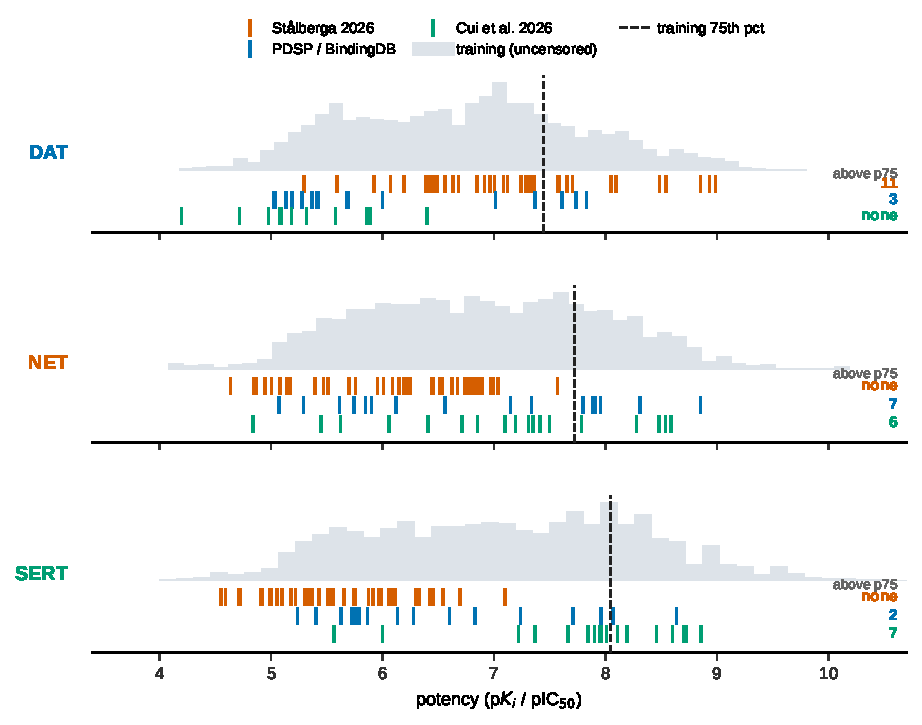
\includegraphics[width=\linewidth]{figures/fig13_newsets.pdf}
\caption{Response-range coverage of the three external sets against the uncensored
training distribution, after removing compounds sharing an InChIKey skeleton block with
training (42, 17 and 20 compounds remain). Ticks are individual compounds; the dashed
line is the training 75th percentile. The advance-specified stimulant panel places no
compound above it at NET or SERT, and eleven at DAT. Of the two later sets, PDSP places 7
and Cui 6 above the line at NET, and 2 and 7 at SERT. The advance-specified stimulant
panel is the only one of the three confined to a single target.}
\label{fig:newsets}
\end{figure}

\FloatBarrier
\section{Discussion}

\paragraph{One failure, three times.} The results above are easier to hold together than
their number suggests, because three of them are the same failure. In each case a pooled
statistic was read as a property of the thing it names, and turned out to be a property of
the composition of the set it was averaged over.

The binding-versus-functional offset at NET reads as a property of the measurement format.
It is a property of the assay cell, indexed here by target and radioligand: $+0.507$ with [$^{125}$I]RTI-55,
$+0.038$ with [$^{3}$H]nisoxetine, and spanning 1.5 log units across the binding assays in
this corpus (\S\,\ref{sec:radioligand-results}). The per-target number is a weighted
average over whichever radioligands dominate that target's literature, and NET looks
special because NET is where the largest-offset cell is most used.

The external $R^2$ reads as a property of the model. It is substantially a property of
where the test compounds sit in the training response distribution: restricting the
training set to the external response region reproduces 53--90\% of the shortfall, and
the achievable ceiling on the advance-specified set is 0.279 at NET against 0.633
internally (\S\,\ref{sec:cannot-evaluate}).

And the composition-matched comparator reads as a property of the model's difficulty. It
does not exist: for all nine cells the external set's composition lies outside what any
internal subset attains, and the sampler that appears to supply one is widening its
tolerance until something is accepted (\S\,\ref{sec:decomp}).

The practical recommendation that follows is one sentence: report what a number was
averaged over --- which assay cells, which response region --- alongside the number, and
check that a comparator exists before interpreting a comparison. Everything else here is
an instance.

\paragraph{What the radioligand result does and does not say.} It does not say the NET
offset is an artefact. The effect is large, replicates across 12 independent documents
within the RTI-55 stratum, and survives a within-document design that removes
between-laboratory calibration. What it says is that ``assay format'' is the wrong name
for it, and therefore the wrong generalisation: a reader who takes a corpus-wide
binding-versus-functional correction from this paper and applies it to a NET dataset
measured with [$^{3}$H]nisoxetine would make the prediction worse, not better. That is
also, finally, a mechanism for the paper's own negative result that a constant correction
failed to transfer. The quantity is not constant. It is near-constant within an assay cell
and varies by more than a log unit between them, which is exactly the condition under
which a pooled correction cannot help.

The confound is not resolved here. Radioligand is collinear with document and nearly with
chemotype in this corpus, and the experiment that would separate them --- the same
compounds at NET by both radioligands in one laboratory --- has not been done. Our claim
is the weaker one that the pooled estimate is an average over heterogeneous cells, which
is enough to invalidate the format reading without establishing the radioligand reading.

\paragraph{Scaffold splitting and the sources.} Scaffold splitting is conservative with
respect to analogue leakage and silent with respect to other sources of external
shortfall. Our decomposition indicates that the dominant one is where the test compounds
sit in the training response distribution, and that source identity contributes little
\emph{unique} variance conditional on the response-range measure included --- 2.1\%.
Because response-range position and source identity are collinear by construction, that is
a statement about this regression and not evidence that laboratory effects are
unimportant.

Chemical novelty performed even more poorly as an explanation. Chemotype matching
reproduced 11--16\% of the shortfall, nearest-neighbour similarity contributed 2.2\%
uniquely, and no external compound lay beyond the training 95th percentile in
descriptor space.

\paragraph{How much stringency does a scaffold split buy?} Two observations here bear
on the wider debate. Measured directly, scaffold splitting cut the proportion of test
compounds with a close training neighbour from 74.5\% to 26.2\% --- a real reduction,
but one that leaves a quarter of the test set with an analogue in training. And for
this target family the Murcko abstraction is a particularly coarse instrument, since
it discards the ring substituents that determine DAT/SERT selectivity: positional
isomers with materially different profiles reduce to the same scaffold. The remedy is
not to abandon scaffold splitting but to report the residual near-neighbour rate
alongside it, and to treat similarity-cluster splitting as the stricter
comparator.\cite{Guo2024,Fooladi2025} We note that the model's features are
substituent-aware even where the splitter is not, so this concerns the stringency of
the evaluation rather than the information available to the model.

\paragraph{Which metric, when.} $R^2$ compares models on a single test set but is
not comparable across test sets of differing response spread, because its reference
is the deviation of observations from their own mean. RMSE measures absolute
accuracy on an interpretable scale and is insensitive to spread, but gives no sense
of whether that accuracy is useful for the range at hand. The $r_m^2$ family was
introduced precisely to bridge this gap \cite{Roy2009,Mitra2010} and remains little
used. Our recommendation is to report RMSE and $R^2$ together with a range-matched
internal comparator, so that a reader can see both the absolute error and how much
of any $R^2$ shortfall is attributable to the test set's position.

\paragraph{Report the ceiling, not only the score.} The point above can be made
quantitative, and we suggest it should be. Measurement heterogeneity caps achievable
$R^2$ at $1-\sigma^2_e/\sigma^2_y$, and because $\sigma^2_y$ is the variance of the
evaluation set, that cap moves when the test set does. Here it falls from 0.633 to
0.279 at NET purely by changing which compounds are being predicted
(Table~\ref{tab:extceiling}). A reader given 0.015 and nothing else will conclude the
model learned nothing; a reader given 0.015 against a reachable 0.279 learns that the
test was close to uninformative before the model was applied, and that the model still
underperformed on what remained. Both conclusions are warranted and only the second is
actionable. The arithmetic requires one quantity that most benchmarks could supply and
few do: an estimate of replicate or cross-modality dispersion on the training endpoint.

The ceiling is not new either. $1-\sigma^2_e/\sigma^2_y$ is the correction for attenuation
due to unreliability, which dates to Spearman and underlies the reliability literature in
psychometrics.\cite{Spearman1904} Naming it matters because the name carries the
assumption: the classical correction treats measurement error as random, independent of
the true value, and mean-zero. The cross-modality dispersion used here is not that. It is
the dispersion \emph{about} a systematic shift --- the mean offset is excluded, so the
shift is not being counted as noise --- but the residual dispersion is itself
heteroscedastic across assay cells, as \S\,\ref{sec:radioligand-results} shows, and the
classical assumption is therefore approximate. Reporting the bound both ways makes the
sensitivity visible: with $\sigma_e$ as the root mean square deviation, which counts the
systematic shift as irreducible, every ceiling falls and the NET ceiling on the
advance-specified set goes to $-0.21$, i.e. no model could score above zero. With
$\sigma_e$ as the SD, as in Table~\ref{tab:extceiling}, it is $+0.279$. The first is too
harsh, since a constant shift is removable in principle; the second is the generous bound
and is the one we report. The true bound lies between, and nothing in this paper's
argument depends on which.

\paragraph{What this means for a forensic or regulatory user.} The Introduction names
that reader, and the paper owes them a plain answer. One cell of this benchmark has
demonstrated external validity: DAT prediction on stimulant-like chemotypes, at
$R^2=0.459$ against a reachable 0.741, which is 62\% of what the measurement noise on that
test set allows. Nothing here supports using a NET or SERT prediction for a novel compound
with any stated confidence: the advance-specified test could not distinguish either from
zero, and the only external set on which both become estimable is a single 20-compound
series from one laboratory. A practical reading is that these models can rank a new
stimulant's DAT potency against known comparators, which is often the question a scheduling
decision turns on, and cannot yet be relied on for the DAT/SERT ratio that separates
stimulant from entactogen character, because the SERT half of that ratio is the half with
no advance-specified external support, and the one exploratory set that does reach it is
the 20-compound series.

\paragraph{A tractable route to NET and SERT coverage.} The scarcity of potent external
NET and SERT data is structural rather than accidental, and the two sets we assembled
afterwards --- neither of them large, and only one of them informative at both
targets --- are the exception that shows how thin the supply is. Assays that yield
single-digit
nanomolar human SERT or NET potencies are run predominantly by medicinal-chemistry
groups publishing in journals that ChEMBL curates comprehensively, so those compounds
become training data rather than test data; the pharmacology and forensic-toxicology
literature that ChEMBL does not systematically curate concerns stimulants, which are
DAT-biased and weak at the other two transporters. That observation also indicates the
remedy. ChEMBL\_37 was released 2026-05-01 with a literature freeze near July 2025, so
any qualifying measurement published after that date is external by construction. A
temporal holdout of this kind requires no new experiments, is immune to the exact-match
and analogue leakage that scaffold splitting only partly controls, and --- unlike the
stimulant panels currently available --- can be assembled specifically to span the
potent end of the NET and SERT range.

\paragraph{Does the model beat its own training data?} For the four compounds
present in both the training set and an independent study, prediction error against
the independent measurement (RMSE 0.878) exceeded the disagreement between the two
laboratories measuring the same molecules (0.683), which in turn exceeded the
model's error against the values it was trained on (0.277). At $n=4$ this is a
design rather than a result, but it frames a question that external validation
rarely asks: whether a model adds information beyond the training measurement
itself. Where inter-laboratory disagreement approaches the apparent generalisation
gap, measurement provenance rather than chemical novelty bounds achievable external
performance. Assembling a larger set of such compounds is a tractable next study.

\paragraph{A measurable difference that is not an actionable one.} The NET
binding-versus-functional offset is the clearest positive result here, and also the
clearest illustration of a gap between detecting an effect and using it. It survives the
controls that hold the laboratory, the mechanism and the value type fixed: within single
publications, within uptake blockers alone, across 49 documents, and after separation from
the $K_i$-versus-IC$_{50}$ component with which ChEMBL confounds it. It does not survive
stratification by radioligand (\S\,\ref{sec:radioligand-results}), which is the control
this paper adds.

And none of the three natural responses recovers any accuracy --- correcting by the
measured constant worsens external fit, training modality-specific models changes internal
accuracy by $+0.002$, and selecting the matching modality at test time costs $-0.017$ once
training-set size is controlled. Two things account for that, and they are different. The
first is within-cell: an offset of $+0.26$ sits inside a compound-to-compound spread of
0.658, so even a correct correction is small relative to the scatter it would be applied
against. The second is between-cell, and is what the radioligand result adds: the quantity
being corrected for is not one quantity. Reviewers of curated bioactivity sets are often
asked to correct for such offsets; this is a case where the offset is real, well
characterised, and still not worth correcting --- and where the reason it cannot be
corrected is also the reason it was mis-named.

\paragraph{Two diagnostics that return a number regardless.} The outcome-conditioned
error regression and the composition-matched comparator fail in the same way and are
worth stating together. In the first, the predictor is computed from the observed
external value and the outcome is computed from the same value, so a regularised model's
shrinkage reproduces the apparent effect with no chemistry involved: $R^2=0.444$ against
a shrinkage null of 0.448, collapsing to 0.001 in the only form available before the
outcome is known. In the second, the comparator is assumed to exist and for none of the
nine cells does it, yet the sampler that constructs it returns a band in every case
because its tolerance widens until one is accepted. Neither failure announces itself. In
both, the diagnostic produces a plausible number whose magnitude is set by the
construction rather than by the data, and in both the check is cheap: compare against a
shrinkage null, and confirm that the matched quantity is attainable before matching on
it. We obtained three mutually inconsistent headline counts from four runs of the second analysis
before running that check, which is the strongest argument we can offer for running it
first.

Five recommendations follow. Report absolute error alongside $R^2$, and consider the
$r_m^2$ metrics designed for this failure mode.\cite{Roy2009} Report a
range-matched internal comparator \emph{and the evidence that one exists}. Report the
position of the external set within the training response distribution. Disaggregate by
source --- not because laboratory identity is itself explanatory, but because pooling
conceals the range heterogeneity that is. And where assay modality is pooled, label it
from the assay description rather than from \texttt{assay\_type}. That field is specific
but insensitive here: it recovers 6\% of the functional measurements the assay text
identifies. The gap is a definitional mismatch --- the field records how the source
publication classified the assay --- rather than curation error, and it is a reason to
read the text, not a criticism of the resource.

\section{Conclusion}

External validation is widely treated as a single binary test that a model either
passes or fails. The present results indicate that the outcome depends heavily on a
property of the test set that is rarely reported: where its compounds sit within the
training response distribution. A model that appears to fail externally may simply have
been evaluated on a narrow slice of its response domain, and one that appears to
succeed may have been evaluated on a favourable one. Neither can be distinguished from
a single $R^2$ value.

At NET and SERT, the external data available when this protocol was fixed contained
no compound potent enough to evaluate a model at all, and the two sets we found
afterwards place the point sharply: one of them restores both targets to significance,
and it is a single 20-compound series. Where a target's informative chemotypes are
absent from the available external data, external validation is not underpowered but
structurally unavailable, and reporting that plainly is more useful than reporting a
coefficient indistinguishable from zero. The corollary is that this condition is a
property of the literature at a moment in time, not of the target, and it can lift ---
which is an argument for stating the coverage alongside the score rather than for
treating any one external result as final.

\section{Limitations}

Five further limitations are declared where they arise rather than here, because each
bears on a specific result: the protocol's self-attested status and its two post hoc
amendments (\S\,\ref{sec:prereg-protocol}); the measured accuracy and the error structure
of the modality classifier (\S\,\ref{sec:modality-labelling}); the overlap filter's
change and what it costs the PDSP set (\S\,\ref{sec:newexternal}); the collinearity of
radioligand with document and chemotype, which is why the stratification identifies a
composition dependence and not a mechanism (\S\,\ref{sec:radioligand-results}); and the
unattainability of a composition-matched comparator in every cell (\S\,\ref{sec:decomp}).
What follows is everything else.

\paragraph{What the external evaluation can support.}
\begin{itemize}\setlength\itemsep{0.15em}
\item The sample could not distinguish null from modest external association at NET and
SERT.
\item The extended evaluation is exploratory; its endpoints were not pre-specified.
\item Two of the four extended sources --- the Luethi and Liechti compilation and the
Basel primary studies --- share a laboratory of origin.
\item The extended external set spans 114 compounds but only 31 Murcko scaffolds
(12, 11, 14 and 3 per source), so the decomposition is established over a narrow slice of
chemical space and its generalisation to more diverse external sets is untested.
\item The nominal spread in $R^2$ across sources did not reach significance ($p=0.065$).
This is a borderline result on four sources and should not be read as demonstrating the
absence of a laboratory effect; per-source estimates are reported for completeness, not as
evidence of one.
\item The source-effect decomposition rests on four studies; the 2.1\% figure indicates
that source adds little beyond range rather than being a precise estimate.
\item The familiar-chemistry comparison has $n=4$ and is a design rather than a result.
\item Conditioning the model on assay modality was tested on the labelled corpus rather
than on the advance-specified benchmark, so that null result is exploratory and shares the
external sets' limited coverage at NET and SERT.
\end{itemize}

\paragraph{The measurement and the curation.}
\begin{itemize}\setlength\itemsep{0.15em}
\item Censored values are carried at their bounds; a full Tobit treatment was not adopted.
\item Seven external compounds were lost to non-determination entries without numeric
bounds.
\item 15.8\% of compounds lie closer to a selectivity class boundary than one replicate
measurement resolves.
\item Murcko scaffolds are a coarse grouping for this target family, since the abstraction
discards the ring substituents that determine selectivity; the scaffold-disjoint folds are
correspondingly a weaker stringency guarantee than the scaffold count alone suggests.
\item Chemotype matching was by compound count rather than by matching the full similarity
distribution.
\end{itemize}

\paragraph{What the offset analysis does not settle.}
\begin{itemize}\setlength\itemsep{0.15em}
\item The offset varies roughly threefold across chemotypes (Kruskal--Wallis across
strata, $p<0.001$). The pooled value is an average over a heterogeneous set, and the
per-stratum samples ($n=5$ to $n=25$) are too small to support a chemotype-resolved
correction.
\item The chemotype stratification was performed on the independently re-retrieved set,
which is non-nested with the frozen one. It therefore tests whether the effect is
chemotype-specific in general, rather than partitioning the frozen estimate.
\item The DAT-versus-SERT comparison is sensitive to retrieval and curation: the two are
not distinguishable in the frozen set ($p=0.39$) but are on an independent re-retrieval
($p=0.005$). Only the contrast between NET and the other two targets is claimed as robust.
\item The fixed-effects decomposition broadens the document base from five papers to 49,
but it still cannot separate assay modality from anything that co-varies with it inside a
single report --- notably substrate concentration and incubation time, which are fixed per
study.
\item The measured offset is established among uptake blockers. The corpus is
overwhelmingly blockers, the structural classifier of \S\,\ref{sec:twobytwo} assigns only
42 compounds as substrate-type, and the offset should not be assumed to transfer to
substrate-type compounds, where the same ratio is one to two orders of magnitude larger.
\item The models predict potency only and do not distinguish transporter substrates from
pure uptake blockers, which is the primary pharmacological distinction for this target
family and is not recoverable from a potency value alone. A criterion based on the ratio
of binding affinity to uptake potency exists \cite{Eshleman2017} but was outside the
advance-specified endpoints, and using it to stratify the offset analysis would be
circular, since that ratio is the quantity under test. Models of these targets that do not
separate the two are predicting a composite endpoint.
\end{itemize}

\paragraph{Inference.}
\begin{itemize}\setlength\itemsep{0.15em}
\item No multiplicity adjustment is applied. The NET-versus-other-targets contrast is the
one confirmatory comparison; every other $p$-value in this paper is exploratory and should
be read as such. The confirmatory contrast survives any correction
($p=1.2\times10^{-8}$ on the re-retrieval, $2.7\times10^{-11}$ on the frozen set); several
exploratory results rest on $p$ between 0.005 and 0.05 and would not.
\item The external-set ceilings in Table~\ref{tab:extceiling} inherit every assumption
behind the dispersion estimates they use: equal error variance in the two modalities,
independent errors, and homoscedasticity across the response range. They are
order-of-magnitude bounds on what a test set of that composition could have shown, not
precise values.
\item Response-range position and source identity are collinear by construction; the
partition separates them statistically but not causally.
\end{itemize}

\section*{Supporting Information}
A companion analysis of structure-based prediction at these targets --- redocking across
nine transporter--ligand complexes, two scoring functions,\cite{Trott2010,Eberhardt2021,Quiroga2016}
cross-docking between conformational states, and pose-derived interaction features ---
reaches conclusions consistent with an independent report using different
software.\cite{Pazos2026}

\section*{List of abbreviations}
DAT: dopamine transporter; NET: norepinephrine transporter; SERT: serotonin
transporter; CCC: concordance correlation coefficient; CI: confidence interval;
ECFP: extended-connectivity fingerprint; IQR: interquartile range; MAE: mean absolute
error; RMSE: root-mean-square error; SD: standard deviation; SEM: standard error of
the mean.

\section*{Declarations}

\subsection*{Availability of data and materials}
The datasets supporting the conclusions of this article are available in the Zenodo
repository, \mbox{\href{https://doi.org/10.5281/zenodo.23144306}{10.5281/zenodo.23144306}}.
The repository contains the curated benchmark
(2849 compounds with per-target potencies, censoring flags, scaffolds and
provenance), the frozen fold assignments, the extended external set with source
attribution, and all analysis code, released under CC~BY~4.0 for data and the MIT
licence for code. The revision additionally deposits the independent re-retrieval
script (\texttt{src/replicate\_assay\_offset.py}), the 16\,750 retrieved activity
records, the per-compound paired NET table, and the chemotype stratification output
in machine-readable form. No registration or licence agreement is required for
access. Bioactivities derive from ChEMBL release 37 (and, for the re-retrieval, from
the live release accessed 2026-09-27); structures from PubChem.

\subsection*{Competing interests}
The author declares no competing interests.

\subsection*{Funding}
This research received no specific grant from any funding agency in the public,
commercial or not-for-profit sectors.

\subsection*{Authors' contributions}
SES conceived the study, curated the data, performed all analyses, produced the
figures, and wrote the manuscript. The author read and approved the final manuscript.

\subsection*{Acknowledgements}
We thank the ChEMBL team at EMBL-EBI, and the authors of the external datasets used
here, whose published primary data made the external evaluation possible.

\subsection*{Implementation errors identified during development}
In the interest of reproducibility we record errors found and corrected before
submission: a protonation routine that left tertiary amines neutral; a use-after-free
in structure preparation producing non-deterministic coordinate corruption; a
misattributed prior-art citation; a reproducibility statistic inflated four-fold by
taking a maximum of ranges rather than a per-target standard deviation; a selectivity
threshold attributed to the wrong publication; a fold-generation function that
silently ignored its random seed; twenty CAS registry numbers leaked across wrapped
table rows during structure resolution; and a database property rename that caused a
structure cross-validation check to return zero comparisons. Each produced plausible
output and raised no error, and all were concentrated in variance estimation,
provenance handling or validation code rather than in point estimates. Automated
regression tests covering each are included in the deposited repository.

A further set was found during revision and each is declared where it bears on a result
rather than only here: one external structure recorded as the wrong molecule, with its two
linked consequences (\S\,\ref{sec:prereg-protocol} and Limitations); an overlap filter
applied on the full InChIKey where the fingerprint ignores stereochemistry, which left 13
compounds of one exploratory set fingerprint-identical to training compounds
(\S\,\ref{sec:newexternal}); a figure that plotted the reciprocal of the regression
whose slope it annotated (Figure~\ref{fig:obspred}); two figure annotations asserting
claims the body retracts; a reproducibility statement claiming three-decimal agreement
across values differing at the third decimal (\S\,\ref{sec:reimplementation}); a structure
file in which two records carried a CXSMILES annotation the default parser rejects,
silently dropping one real compound; and several arithmetic slips in counts and
standard-deviation ratios. The pattern is the same as above --- each produced plausible
output and none raised an error --- and the two that changed a reported result, the
overlap filter and the radioligand stratification of \S\,\ref{sec:radioligand-results},
both moved it against the paper's prior claim.

\bibliography{references}

\end{document}
